\chapter{7 TeV and 8 TeV Differential Cross Section Measurement: Fitting, Unfolding and Measurement}
\label{c:Differential_Cross_Section:fitting_and_unfolding}

% \section{Introduction}
% \label:{s:analysis2_introduction}
% Following event selection it is important to perform a comparison of simulation to data to verify that the
% processes modelled as backgrounds 

\section{Data-MC Comparison}
\label{ss:data-mc_comparison}
Following the full event selection, the distributions of the primary variables \met, \HT, \st, \wpt and \mt
are shown in Figures \ref{fig:data_mc_comparison_7TeV_electron} and \ref{fig:data_mc_comparison_7TeV_muon} for
the electron and muon channels respectively at $\sqrt{s}=7\TeV$; and in Figures
\ref{fig:data_mc_comparison_8TeV_electron} and \ref{fig:data_mc_comparison_8TeV_muon} respectively at
$\sqrt{s}=8\TeV$. The normalisations and shapes are all obtained form simulation except in the case of QCD
which is taken from data: the conversion region is used in the electron channel and the non-isolated region is
used in the muon channel. In general, the agreement between data and simulation is good, with the
distributions simulation peaking at slightly higher energies because event reweighting to account for the \pt
mismodelling of the top quark in simulation has not yet been carried out at this stage.

\begin{figure}[hbtp]
    \centering
     \includegraphics[width=0.48\textwidth]{Chapters/04_Analysis/04b_XSections/images/control_plots/before_fit/7TeV/EPlusJets_patType1CorrectedPFMet_2orMoreBtags_with_ratio.pdf}\hfill
     \includegraphics[width=0.48\textwidth]{Chapters/04_Analysis/04b_XSections/images/control_plots/before_fit/7TeV/EPlusJets_HT_2orMoreBtags_with_ratio.pdf}\\
     \includegraphics[width=0.48\textwidth]{Chapters/04_Analysis/04b_XSections/images/control_plots/before_fit/7TeV/EPlusJets_patType1CorrectedPFMet_ST_2orMoreBtags_with_ratio.pdf}\hfill
     \includegraphics[width=0.48\textwidth]{Chapters/04_Analysis/04b_XSections/images/control_plots/before_fit/7TeV/EPlusJets_patType1CorrectedPFMet_WPT_2orMoreBtags_with_ratio.pdf}\\
     \includegraphics[width=0.48\textwidth]{Chapters/04_Analysis/04b_XSections/images/control_plots/before_fit/7TeV/EPlusJets_patType1CorrectedPFMet_MT_2orMoreBtags_with_ratio.pdf}\hfill
     \caption{Comparison of Monte Carlo simulation to data in the electron+jets channel after final
     selection at $\sqrt{s}=7\TeV$.}
     \label{fig:data_mc_comparison_7TeV_electron}
\end{figure}

\begin{figure}[hbtp]
    \centering
     \includegraphics[width=0.48\textwidth]{Chapters/04_Analysis/04b_XSections/images/control_plots/before_fit/7TeV/MuPlusJets_patType1CorrectedPFMet_2orMoreBtags_with_ratio.pdf}\hfill
     \includegraphics[width=0.48\textwidth]{Chapters/04_Analysis/04b_XSections/images/control_plots/before_fit/7TeV/MuPlusJets_HT_2orMoreBtags_with_ratio.pdf}\\
     \includegraphics[width=0.48\textwidth]{Chapters/04_Analysis/04b_XSections/images/control_plots/before_fit/7TeV/MuPlusJets_patType1CorrectedPFMet_ST_2orMoreBtags_with_ratio.pdf}\hfill
     \includegraphics[width=0.48\textwidth]{Chapters/04_Analysis/04b_XSections/images/control_plots/before_fit/7TeV/MuPlusJets_patType1CorrectedPFMet_WPT_2orMoreBtags_with_ratio.pdf}\\
     \includegraphics[width=0.48\textwidth]{Chapters/04_Analysis/04b_XSections/images/control_plots/before_fit/7TeV/MuPlusJets_patType1CorrectedPFMet_MT_2orMoreBtags_with_ratio.pdf}\hfill
     \caption{Comparison of Monte Carlo simulation to data in the muon+jets channel after final
     selection at $\sqrt{s}=7\TeV$.}
     \label{fig:data_mc_comparison_7TeV_muon}
\end{figure}
 
\begin{figure}[hbtp]
    \centering
     \includegraphics[width=0.48\textwidth]{Chapters/04_Analysis/04b_XSections/images/control_plots/before_fit/8TeV/EPlusJets_patType1CorrectedPFMet_2orMoreBtags_with_ratio.pdf}\hfill
     \includegraphics[width=0.48\textwidth]{Chapters/04_Analysis/04b_XSections/images/control_plots/before_fit/8TeV/EPlusJets_HT_2orMoreBtags_with_ratio.pdf}\\
     \includegraphics[width=0.48\textwidth]{Chapters/04_Analysis/04b_XSections/images/control_plots/before_fit/8TeV/EPlusJets_patType1CorrectedPFMet_ST_2orMoreBtags_with_ratio.pdf}\hfill
     \includegraphics[width=0.48\textwidth]{Chapters/04_Analysis/04b_XSections/images/control_plots/before_fit/8TeV/EPlusJets_patType1CorrectedPFMet_WPT_2orMoreBtags_with_ratio.pdf}\\
     \includegraphics[width=0.48\textwidth]{Chapters/04_Analysis/04b_XSections/images/control_plots/before_fit/8TeV/EPlusJets_patType1CorrectedPFMet_MT_2orMoreBtags_with_ratio.pdf}\hfill
     \caption{Comparison of Monte Carlo simulation to data in the electron+jets channel after final
     selection at $\sqrt{s}=8\TeV$.}
     \label{fig:data_mc_comparison_8TeV_electron}
\end{figure}
 
\begin{figure}[hbtp]
    \centering
     \includegraphics[width=0.48\textwidth]{Chapters/04_Analysis/04b_XSections/images/control_plots/before_fit/8TeV/MuPlusJets_patType1CorrectedPFMet_2orMoreBtags_with_ratio.pdf}\hfill
     \includegraphics[width=0.48\textwidth]{Chapters/04_Analysis/04b_XSections/images/control_plots/before_fit/8TeV/MuPlusJets_HT_2orMoreBtags_with_ratio.pdf}\\
     \includegraphics[width=0.48\textwidth]{Chapters/04_Analysis/04b_XSections/images/control_plots/before_fit/8TeV/MuPlusJets_patType1CorrectedPFMet_ST_2orMoreBtags_with_ratio.pdf}\hfill
     \includegraphics[width=0.48\textwidth]{Chapters/04_Analysis/04b_XSections/images/control_plots/before_fit/8TeV/MuPlusJets_patType1CorrectedPFMet_WPT_2orMoreBtags_with_ratio.pdf}\\
     \includegraphics[width=0.48\textwidth]{Chapters/04_Analysis/04b_XSections/images/control_plots/before_fit/8TeV/MuPlusJets_patType1CorrectedPFMet_MT_2orMoreBtags_with_ratio.pdf}\hfill
     \caption{Comparison of Monte Carlo simulation to data in the muon+jets channel after final
     selection at $\sqrt{s}=8\TeV$.}
     \label{fig:data_mc_comparison_8TeV_muon}
\end{figure}

A comparison between data and simulation in the electron+jets QCD selections is shown in
Figure~\ref{fig:data_mc_comparison_electron_QCD}. There is reasonably good agreement between the data and
simulation in the conversion selection but low statistics in the $\sqrt{s}=8\TeV$ simulation lead to some
events with large weights, leading to peaks in the distribution. It can also be seen that there are more
conversion events in the regions of the endcaps, where the larger amount of detector material for electrons to
traverse leads to a higher number of conversions. The non-isolated QCD selection shows more discrepancies
between the simulation and data, but it should be noted that at $\sqrt{s}=7\TeV$ the simulation does not
contain the triggers used in this analysis, unlike at $\sqrt{s}=8\TeV$, therefore the simulation distirbution
at $\sqrt{s}=7\TeV$ is not affected by the trigger isolation requirements.

The true QCD background distribution is a mixture of the conversion and non-isolated distributions. A
comparison of the two QCD background selections at $\sqrt{s}=7\TeV$ and $\sqrt{s}=8\TeV$ is also shown in
Figure~\ref{fig:data_mc_comparison_electron_QCD}. Background events in which electrons come from jets
misreconstructed as electrons or from \bquark or \cquark decays will pass the non-isolated selection, whereas
conversion events in which the second electron is not rejected by the electron veto will pass the conversion
selection. Another point to note is that, while the general shape of the conversion selection is expected to
be the same in both signal and QCD background selections, the same may not be true of the non-isolated
selection due to the isolation requirement in the signal selection. In addition, the number of events passing
the QCD background selections will be very small compared to the number of events passing the signal
selection, so the effect of even large uncertainties in the QCD background on the total number of events
will be minimal.

In the muon+jets channel, again it is clear that the data and simulation are not in agreement and that there
is a low amount of statistics available in simulation.

 \begin{figure}[hbtp]
    \centering
%      \includegraphics[width=0.48\textwidth]{Chapters/04_Analysis/04b_XSections/images/control_plots/before_fit/7TeV/}\hfill
%      \includegraphics[width=0.48\textwidth]{Chapters/04_Analysis/04b_XSections/images/control_plots/before_fit/8TeV/}\\
%      \includegraphics[width=0.48\textwidth]{Chapters/04_Analysis/04b_XSections/images/control_plots/before_fit/7TeV/}\hfill
%      \includegraphics[width=0.48\textwidth]{Chapters/04_Analysis/04b_XSections/images/control_plots/before_fit/8TeV/}\\
%      \includegraphics[width=0.48\textwidth]{Chapters/04_Analysis/04b_XSections/images/control_plots/before_fit/7TeV/}\hfill
%      \includegraphics[width=0.48\textwidth]{Chapters/04_Analysis/04b_XSections/images/control_plots/before_fit/7TeV/}\\
     
\includegraphics[width=0.48\textwidth]{Chapters/04_Analysis/04b_XSections/images/placeholder.png}\hfill
     
\includegraphics[width=0.48\textwidth]{Chapters/04_Analysis/04b_XSections/images/placeholder.png}\\
     
\includegraphics[width=0.48\textwidth]{Chapters/04_Analysis/04b_XSections/images/placeholder.png}\hfill
     
\includegraphics[width=0.48\textwidth]{Chapters/04_Analysis/04b_XSections/images/placeholder.png}\\
     
\includegraphics[width=0.48\textwidth]{Chapters/04_Analysis/04b_XSections/images/placeholder.png}\hfill
     
\includegraphics[width=0.48\textwidth]{Chapters/04_Analysis/04b_XSections/images/placeholder.png}\\
     \caption{Comparison of QCD selections in the electron+jets channel at $\sqrt{s}=7\TeV$ on the left
     and at $\sqrt{s}=8\TeV$ on the right. Conversion region is shown at the top, non-isolated selection
     in the middle and a comparison of the two selections in data (TODO:CHECK THIS, AND INSERT THE PLOTS IN
     THE FIRST PLACE!)
     %TODO:CHECK THIS
     is shown in the lower plots.}
     \label{fig:data_mc_comparison_electron_QCD}
 \end{figure}

\section{Binning Choice}
\label{s:binning_choice}
The bin boundaries in the primary variable distributions is important because events generated in one bin can
migrate to another bin after reconstrution due to the finite resolution of the detector. This altering of the
number of events, either as a result of events moving into, or out of, a bin is important to understand so
that the final reconstructed distribution can be deconvoluted (unfolded) to the true distribution.

In light of this, the binning choice is made based on two variables defined as purity ($p^k$) and stability
($s^k$):

\begin{eqnarray}
\label{eq:purity_and_stability}
p^k = \frac{N_{\rec\&\gen}^k}{N_{\rec}^k}
s^k = \frac{N_{\rec\&\gen}^k}{N_{\gen}^k}
,
\end{eqnarray}

$N_{\rec\&\gen}^k$ is the number of events generated and reconstructed in bin $k$,
$N_{\rec}^k$ is the number of events reconstructed in bin $k$ and $N_{\gen}^k$ is the number of events
generated in bin $k$. The stability of a bin is sensitive to the migration of events out of a bin, while
the purity is sensitive to the migration of events into a bin (see Figure~\ref{fig:purity_and_stability}.

\begin{figure}[hbtp]
	\centering
     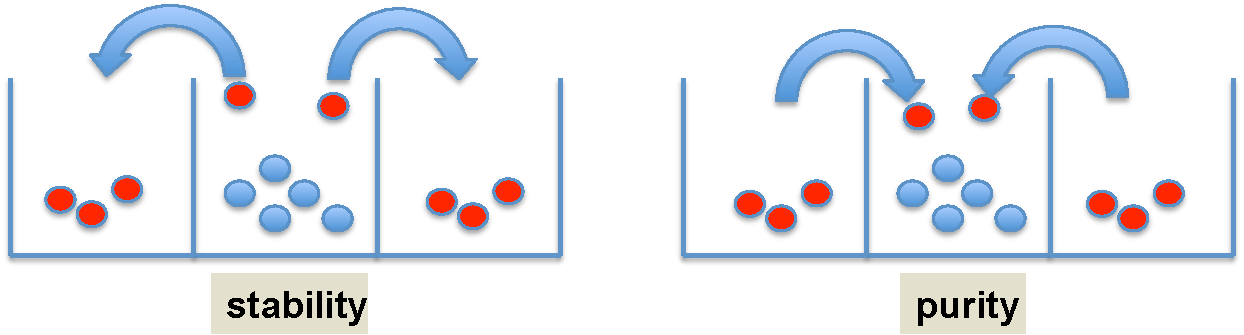
\includegraphics[width=0.8\textwidth]{Chapters/04_Analysis/04b_XSections/images/purity_and_stability.pdf}
     \caption{Stability quantifies the migration of events out of a bin while purity quantifies the migration
     of events into a bin. Both quantities compare the variable range (bin) in which an event is generated to
     the range in which they are reconstructed.}
     \label{fig:purity_and_stability}
 \end{figure}

In this analysis, the bins for each primary variable distribution were chosen such that all bins have purity
and stability values of 0.5 or greater, meaning that at least half of the events generated in a bin remain in that bin
after reconstruction, and that at least half of the events reconstructed in a bin were generated in that bin.
In order to avoid very small bins, a requirement that all bins have at least 100 events is also enforced.

The determination of the bin boundaries following these criteria is carried out simultaneously in (and
therefore the binning is identical in) both centre of mass energies and both the electron+jets and
muon+jets channel.

Plots of generated versus reconstructed events for all primary variables are shown in the electron+jets
channel in Figure~\ref{fig:binning_7TeV_electron} for $\sqrt{s}=7\TeV$ and in
Figure~\ref{fig:binning_8TeV_electron} for $\sqrt{s}=8\TeV$. The corresponding plots in the muon+jets are
shown in Figures~\ref{fig:binning_7TeV_muon} and \ref{fig:binning_8TeV_muon} in
Appendix~\ref{as:binning_muon}. The purity and stability values of the chosen bins are shown in
Appendix~\ref{as:binning_tables_electron}.

\begin{figure}[hbtp]
	\centering
     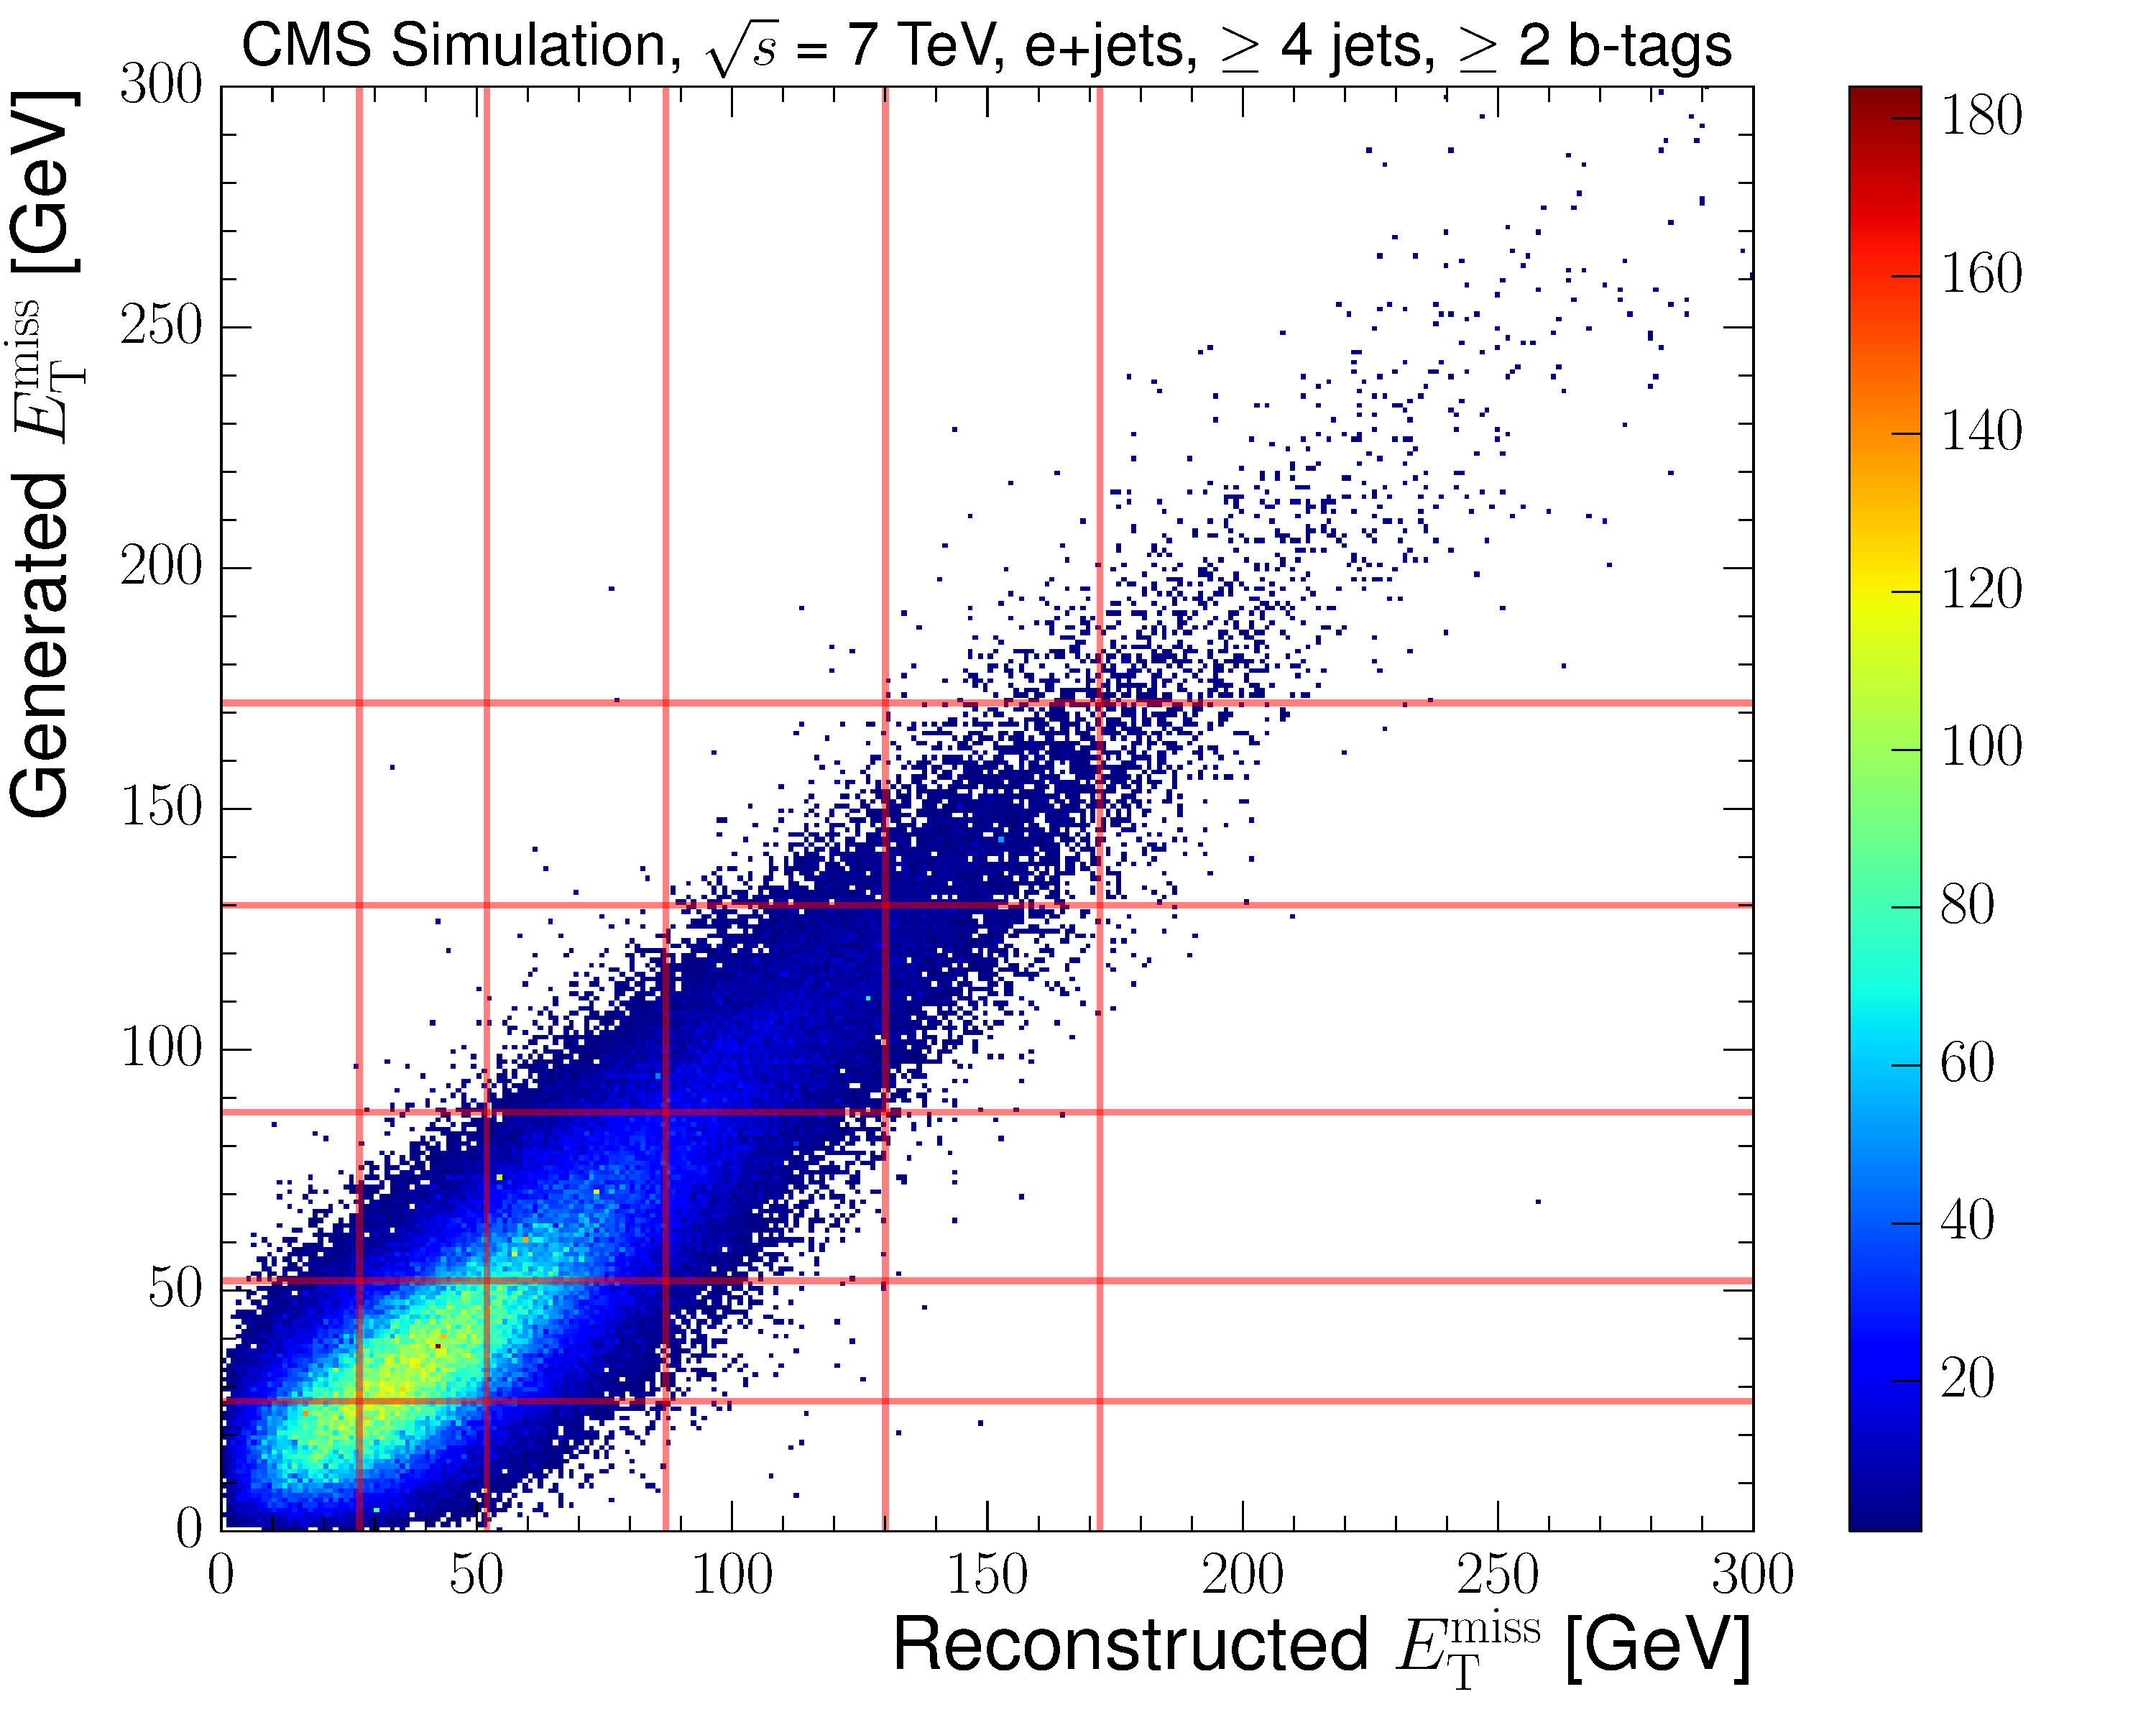
\includegraphics[width=0.48\textwidth]{Chapters/04_Analysis/04b_XSections/images/binning/electron_MET_7TeV.pdf}\hfill
     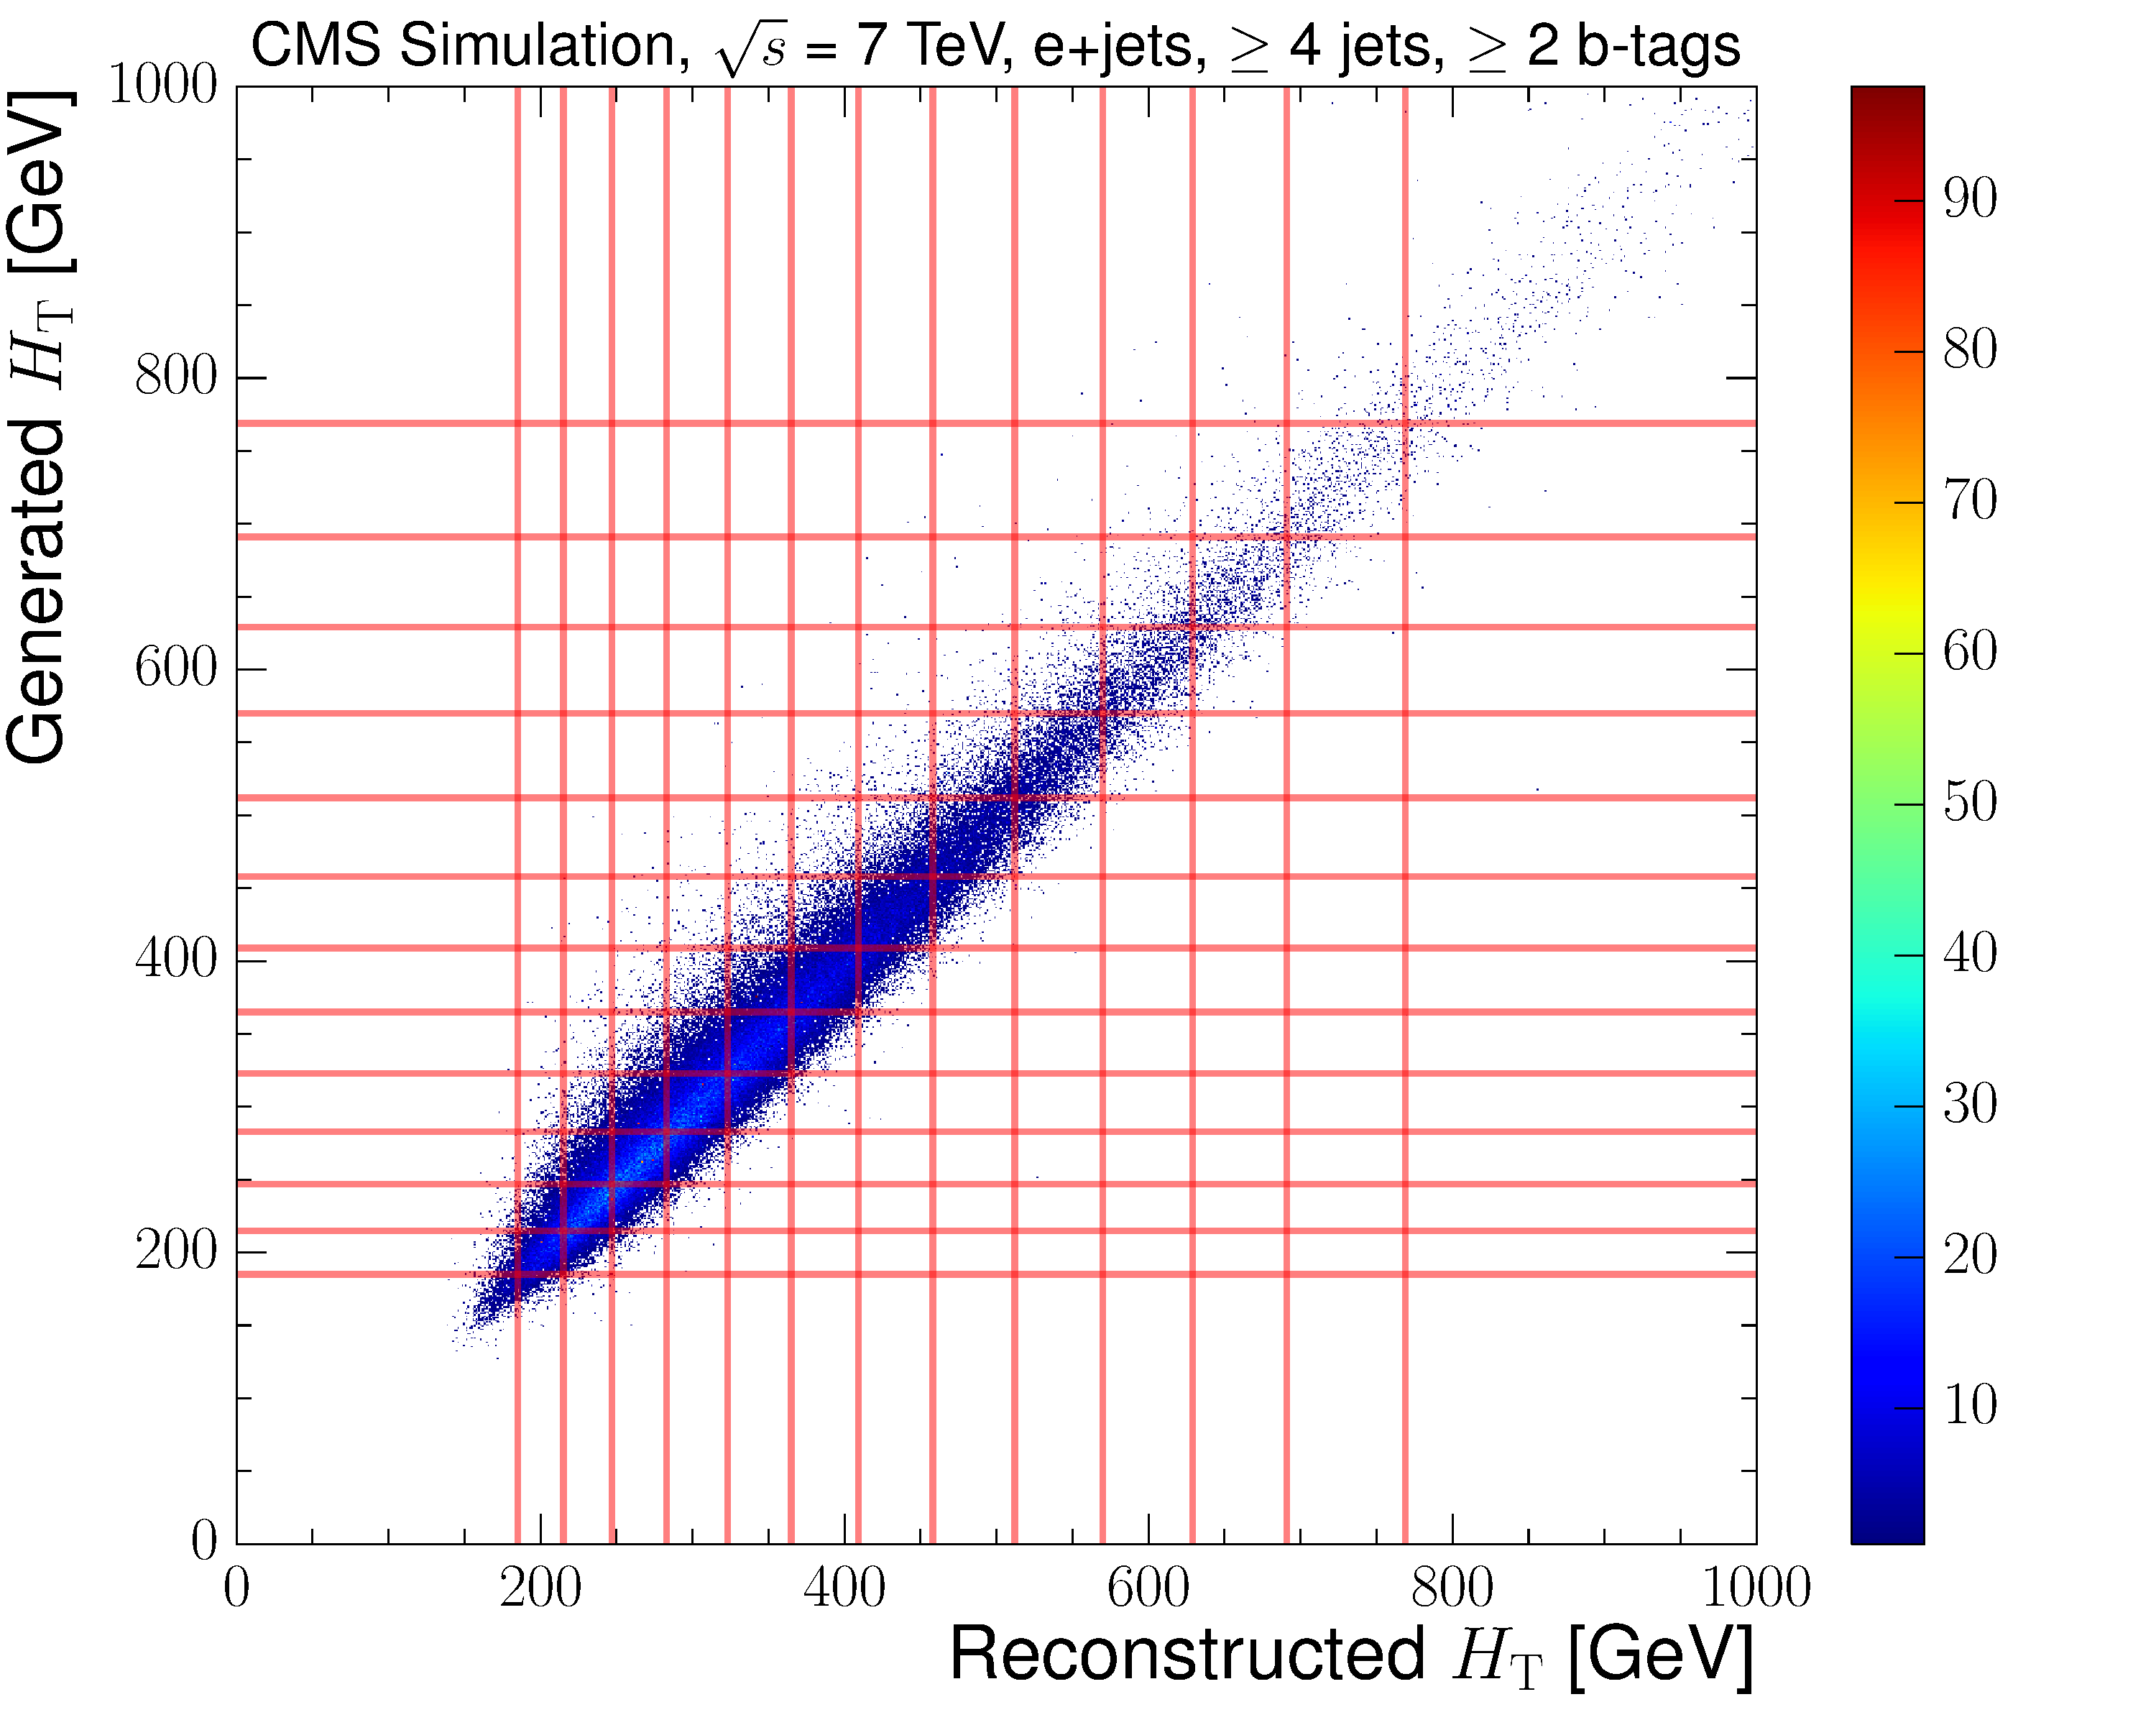
\includegraphics[width=0.48\textwidth]{Chapters/04_Analysis/04b_XSections/images/binning/electron_HT_7TeV.pdf}\\
     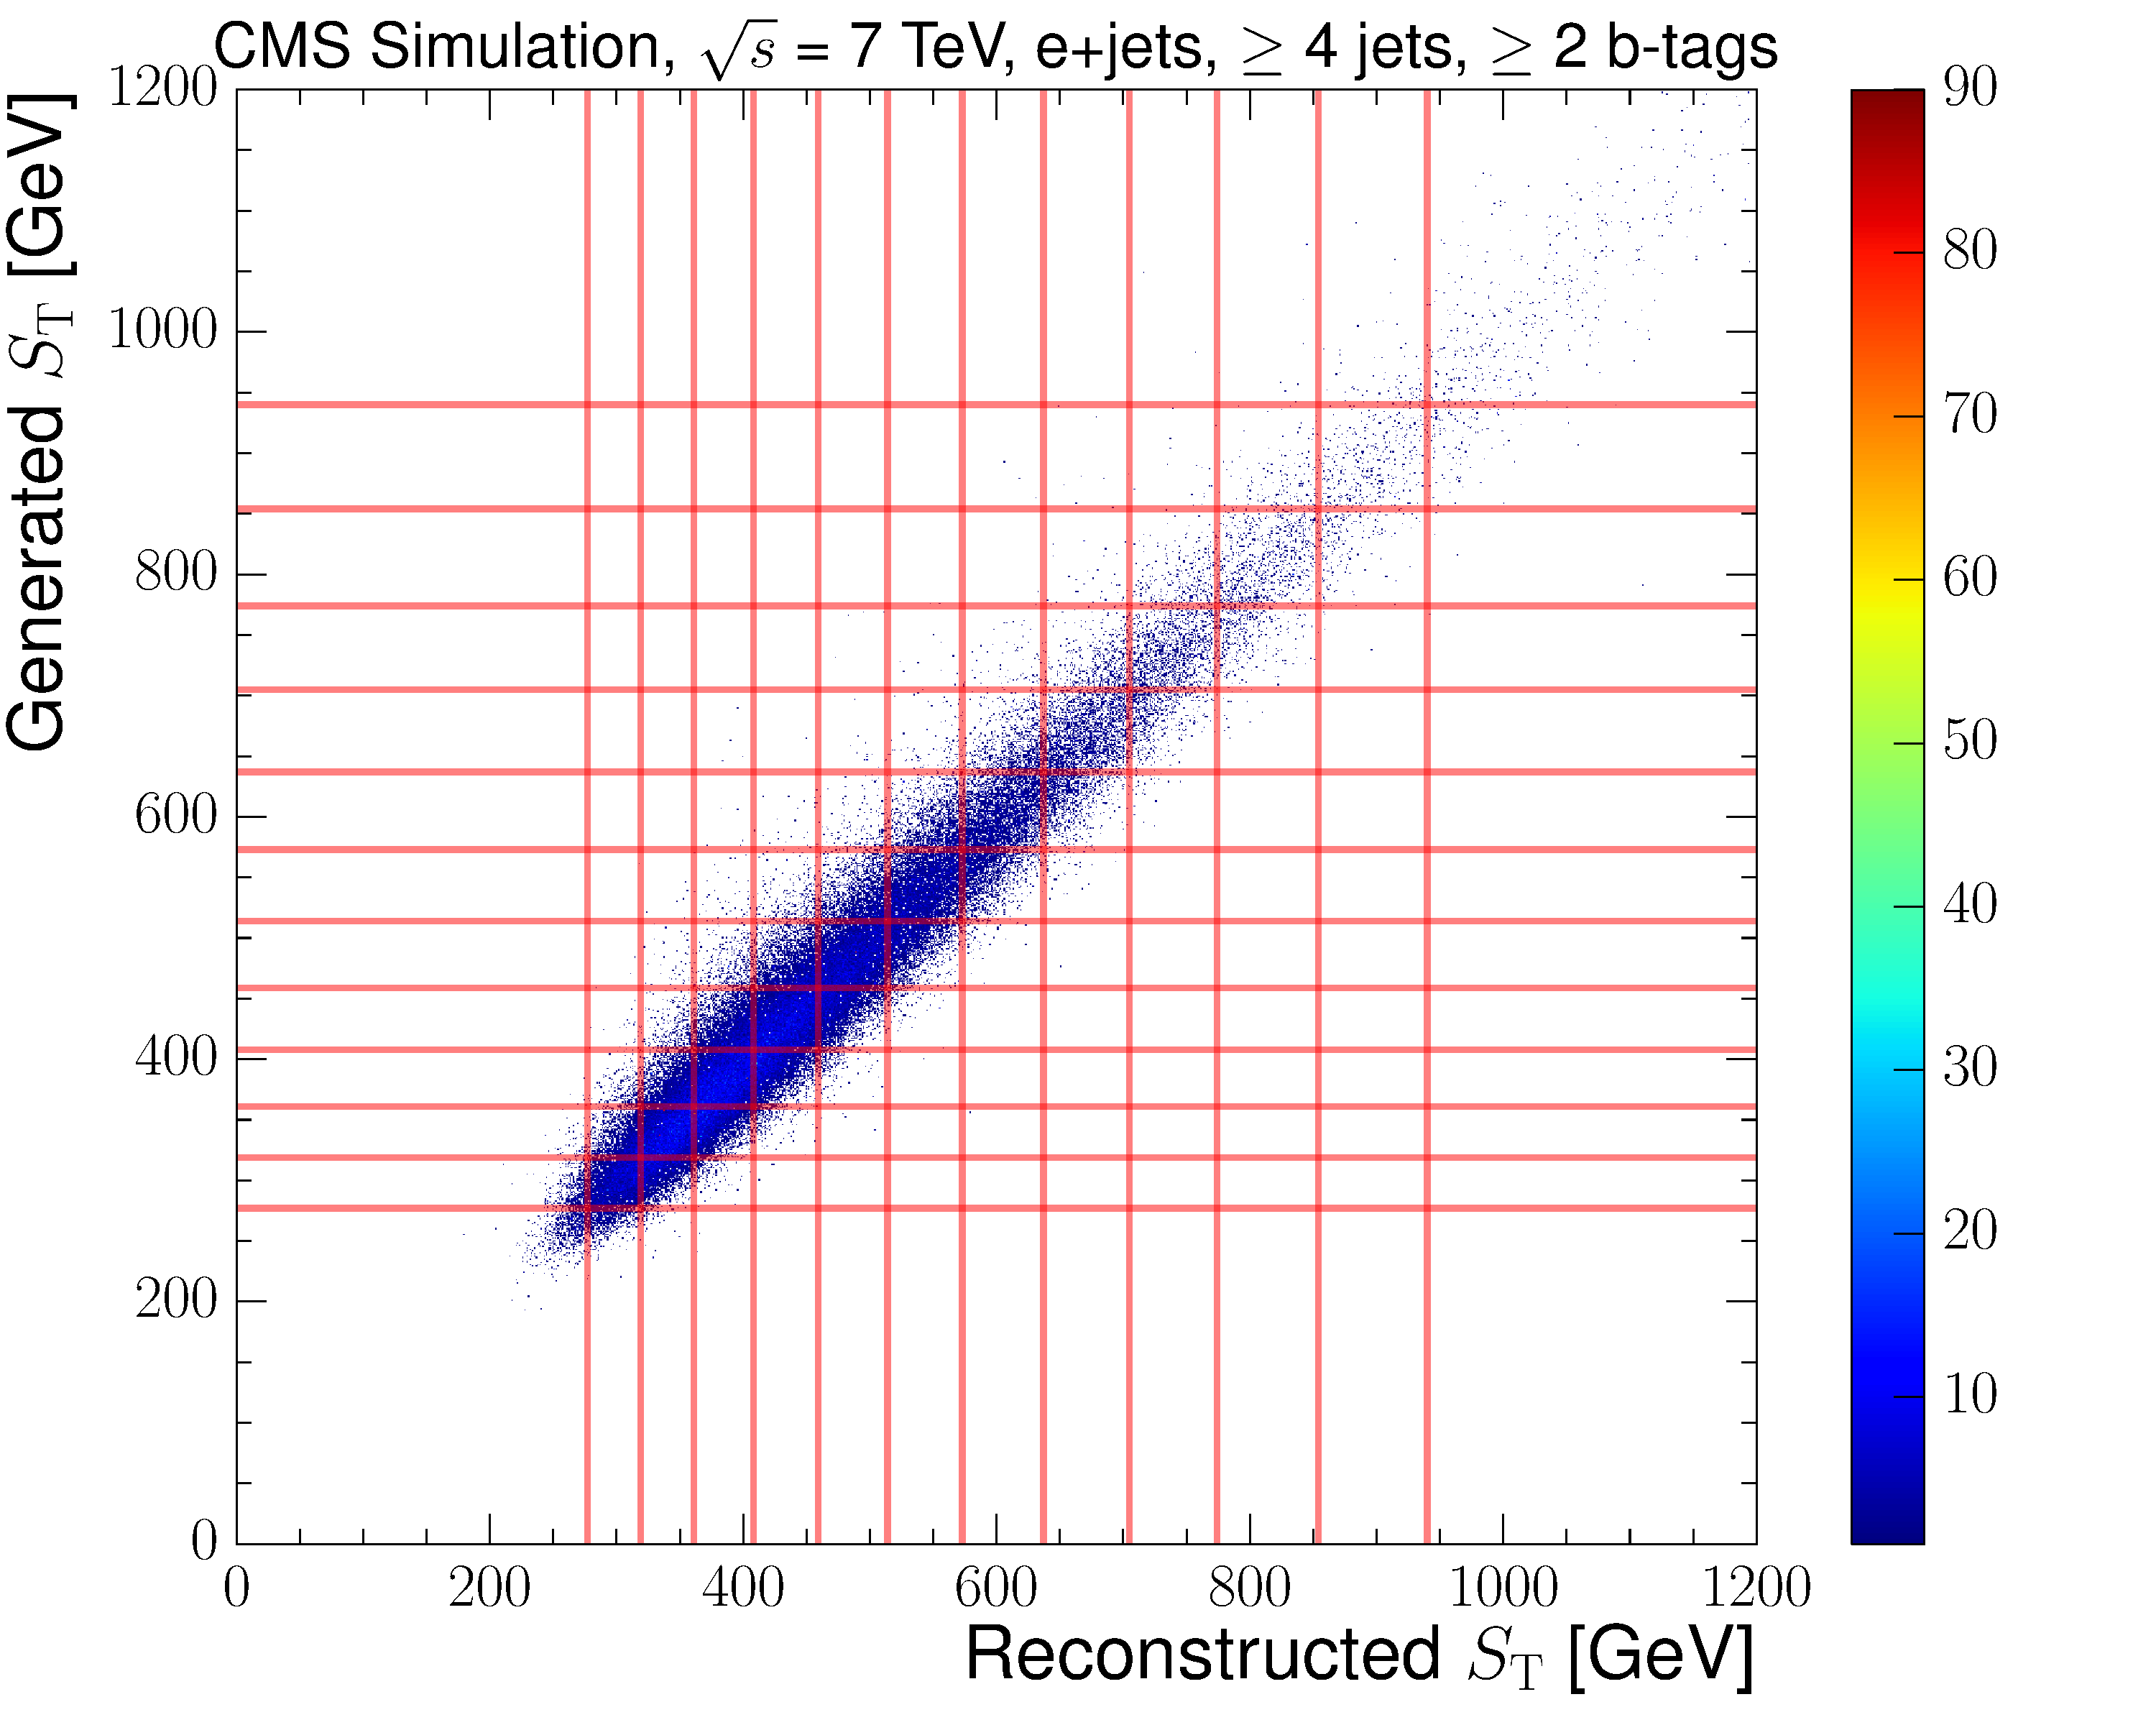
\includegraphics[width=0.48\textwidth]{Chapters/04_Analysis/04b_XSections/images/binning/electron_ST_7TeV.pdf}\hfill
     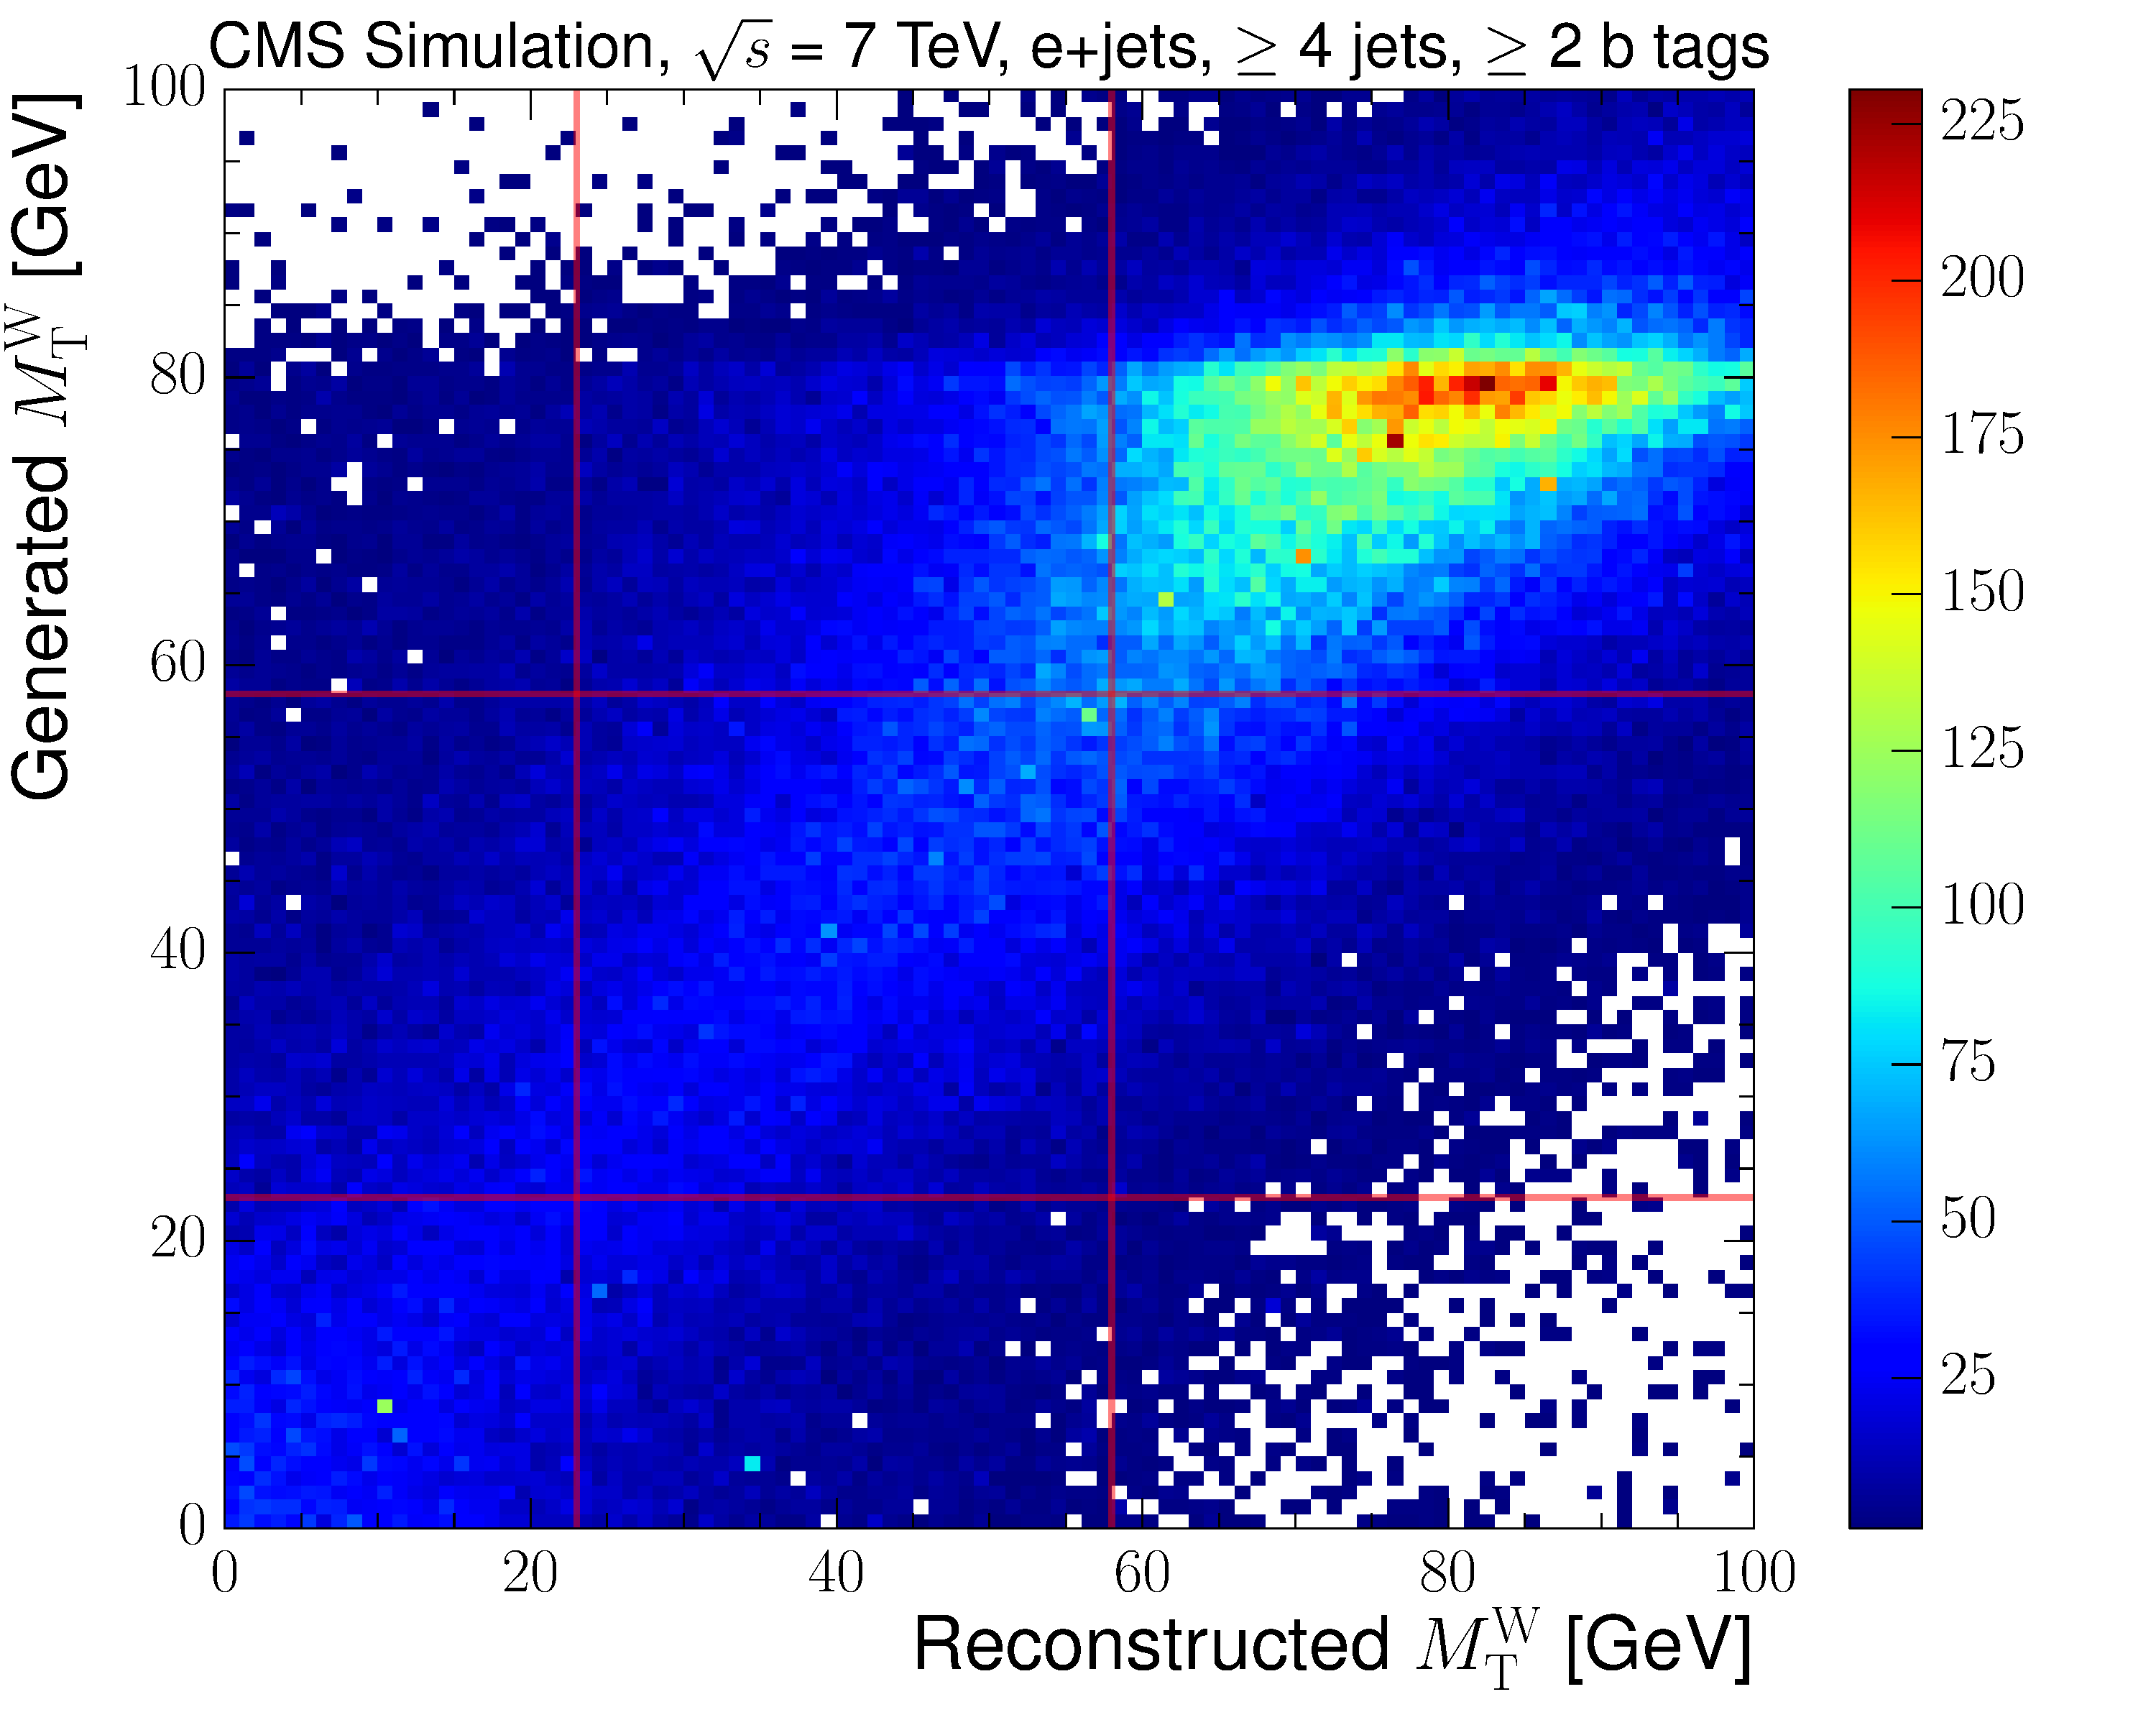
\includegraphics[width=0.48\textwidth]{Chapters/04_Analysis/04b_XSections/images/binning/electron_MT_7TeV.pdf}\\
	 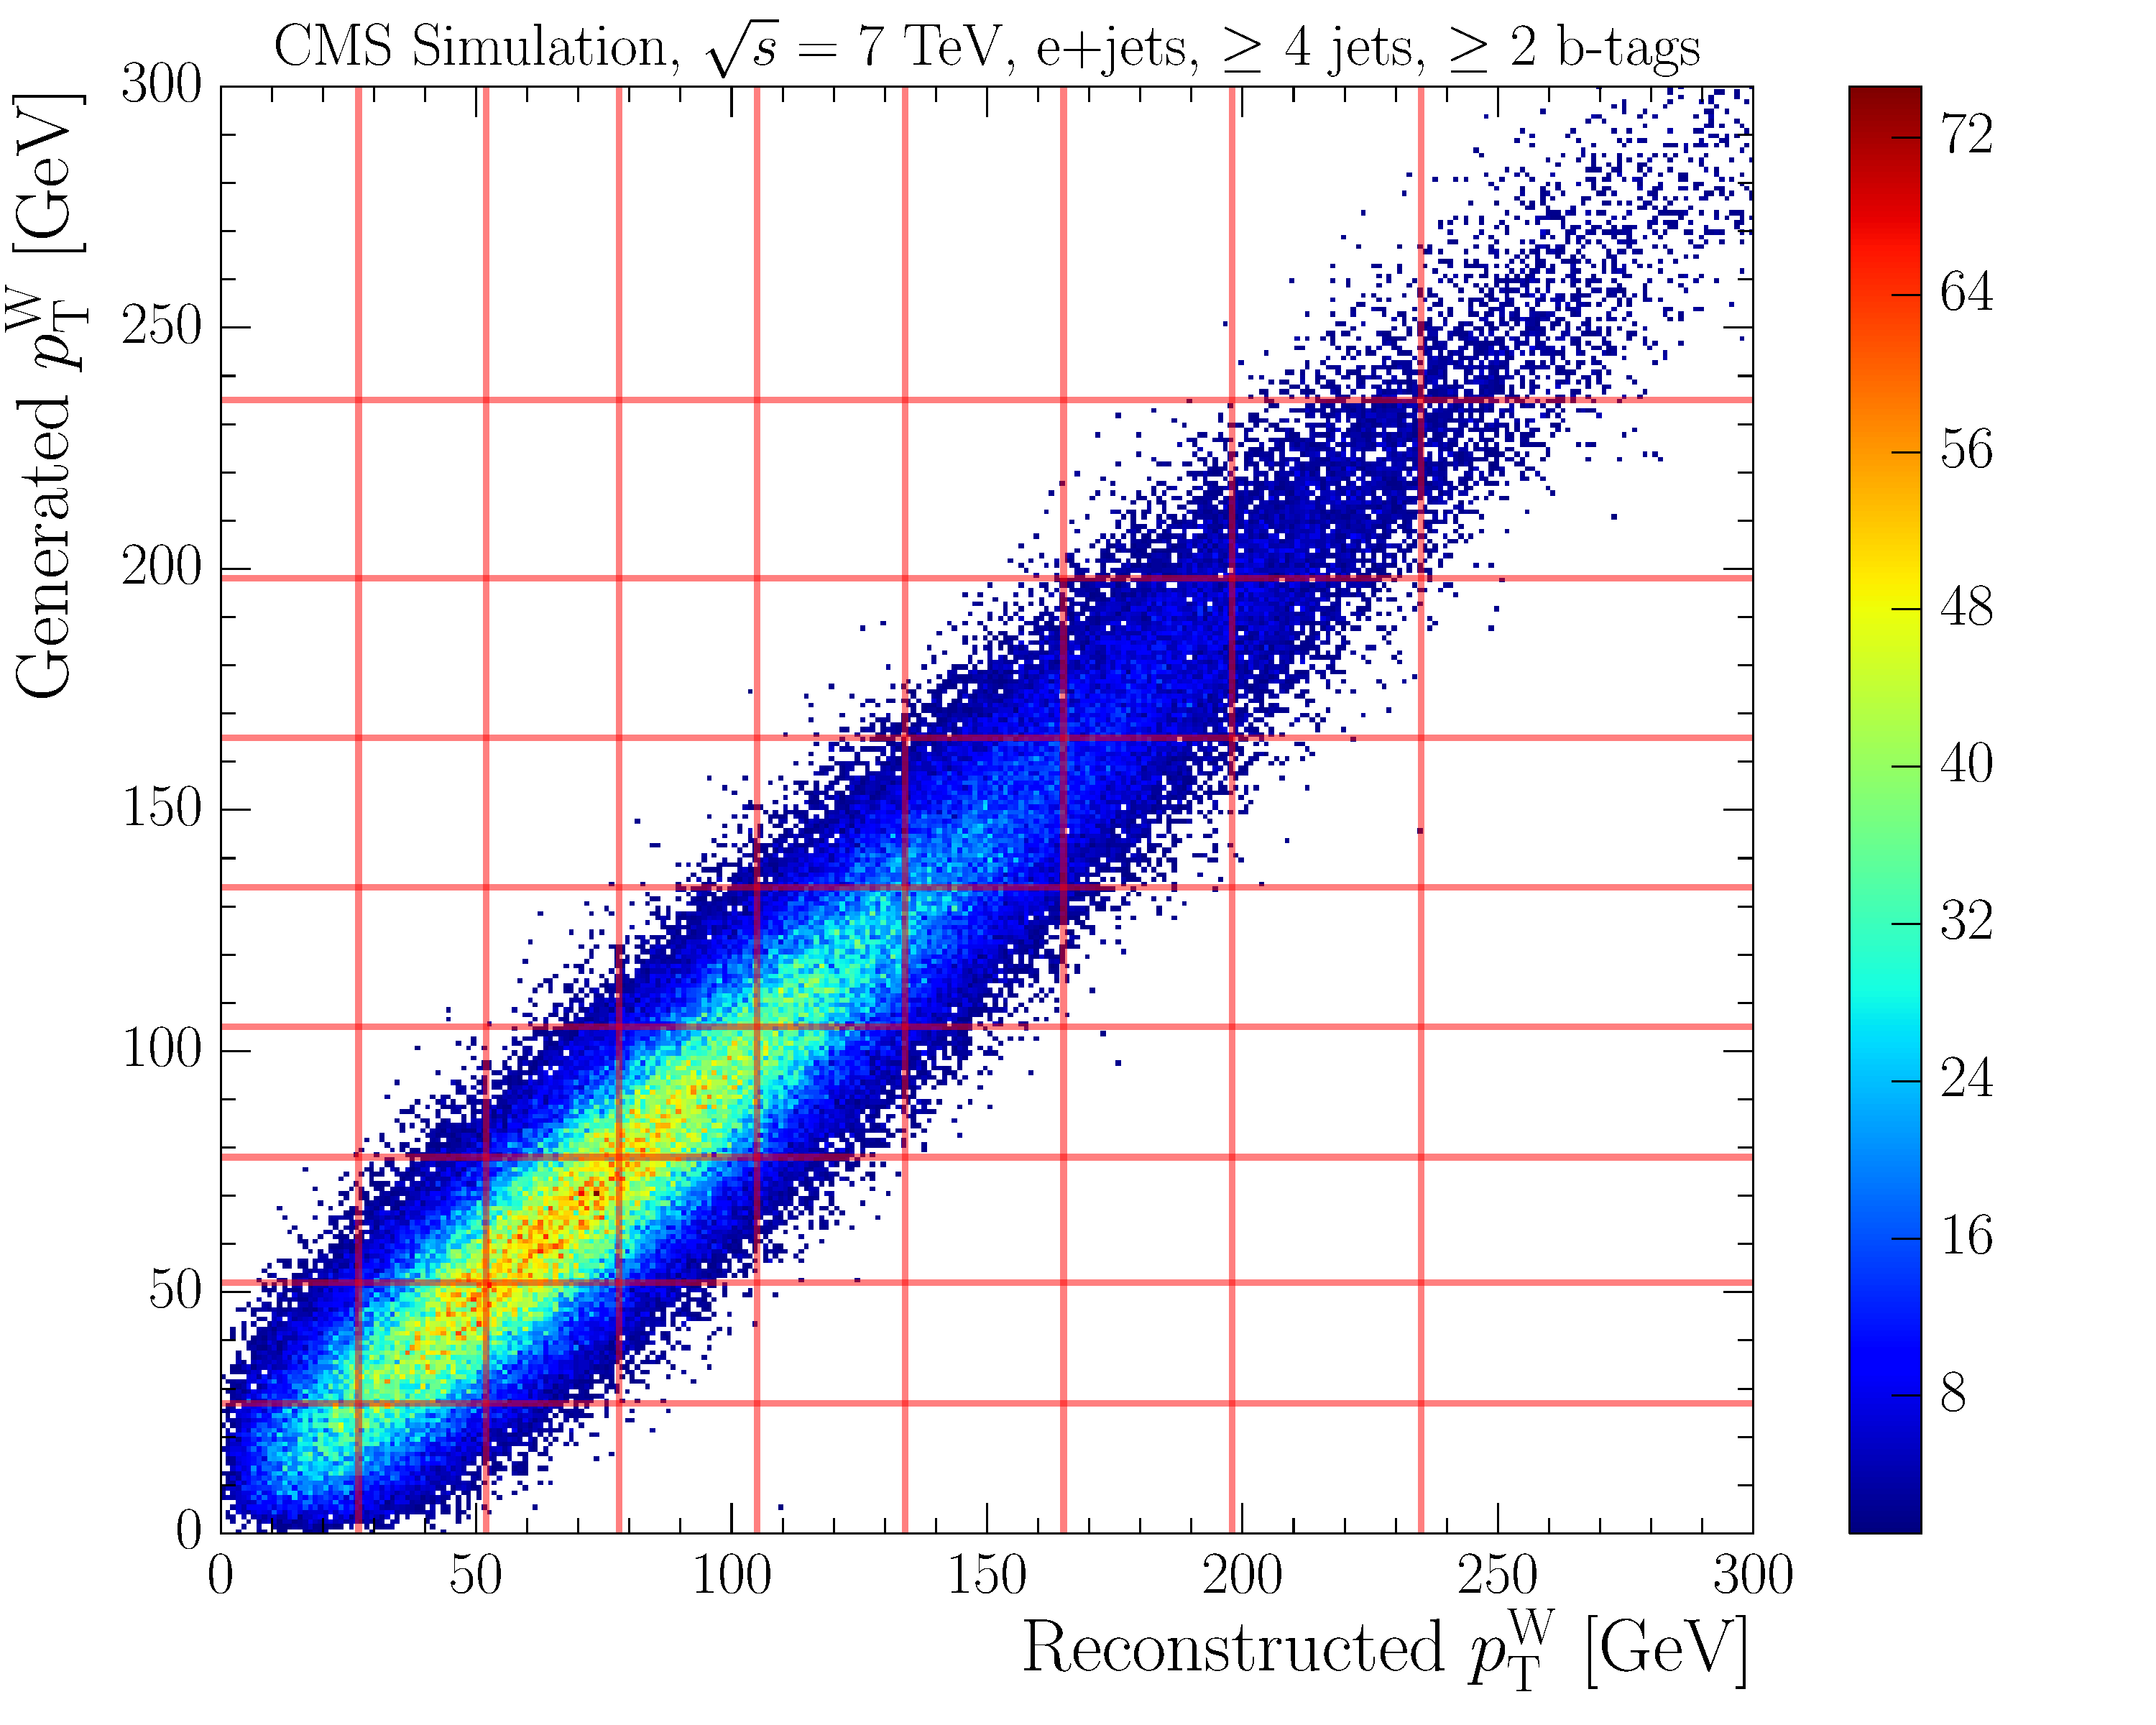
\includegraphics[width=0.48\textwidth]{Chapters/04_Analysis/04b_XSections/images/binning/electron_WPT_7TeV.pdf}\hfill
	 \caption{Generated versus reconstructed distributions of the primary variables \met (upper left), \HT (upper
	 right), \st (middle left), \mt (middle right) and \wpt (lower) with horizontal and vertical lines
	 representing the boundaries of the selected bins at $\sqrt{s}=7\TeV$ in the electron+ jets channel. These
	 distributions are obtained using \ttbar Monte Carlo simulation.}
     \label{fig:binning_7TeV_electron}
\end{figure}

\begin{figure}[hbtp]
    \centering
     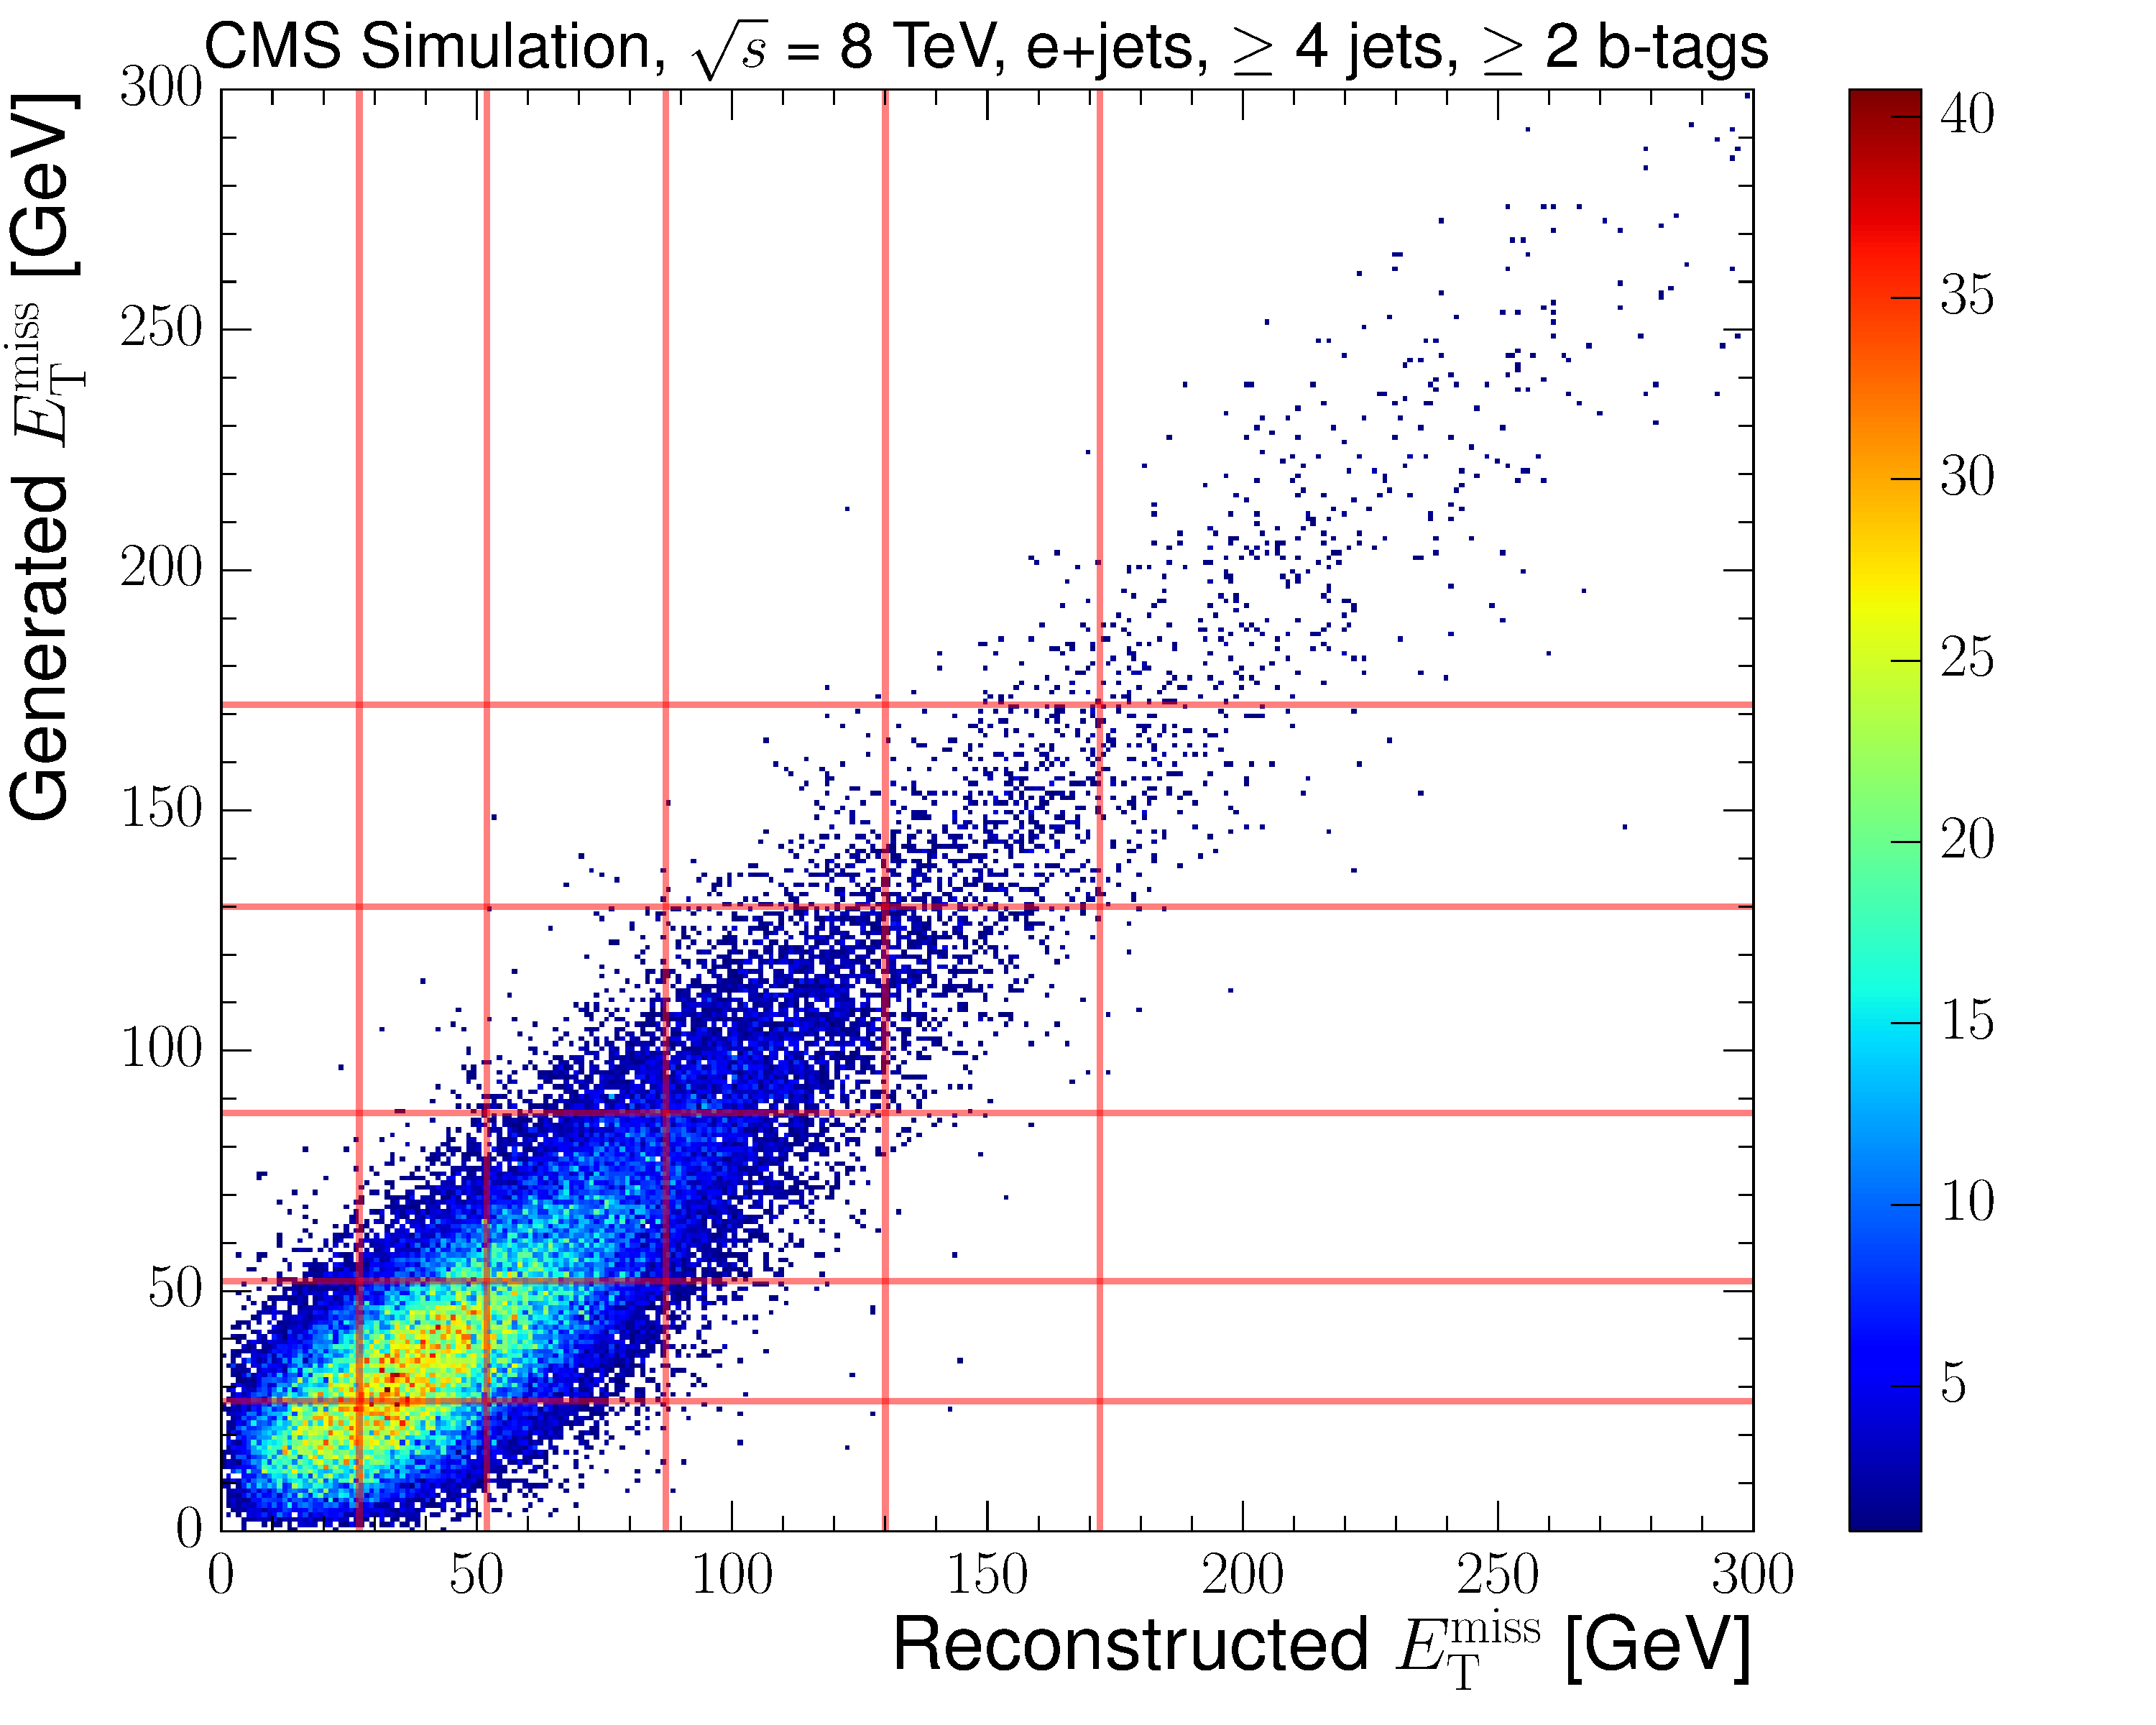
\includegraphics[width=0.48\textwidth]{Chapters/04_Analysis/04b_XSections/images/binning/electron_MET_8TeV.pdf}\hfill
     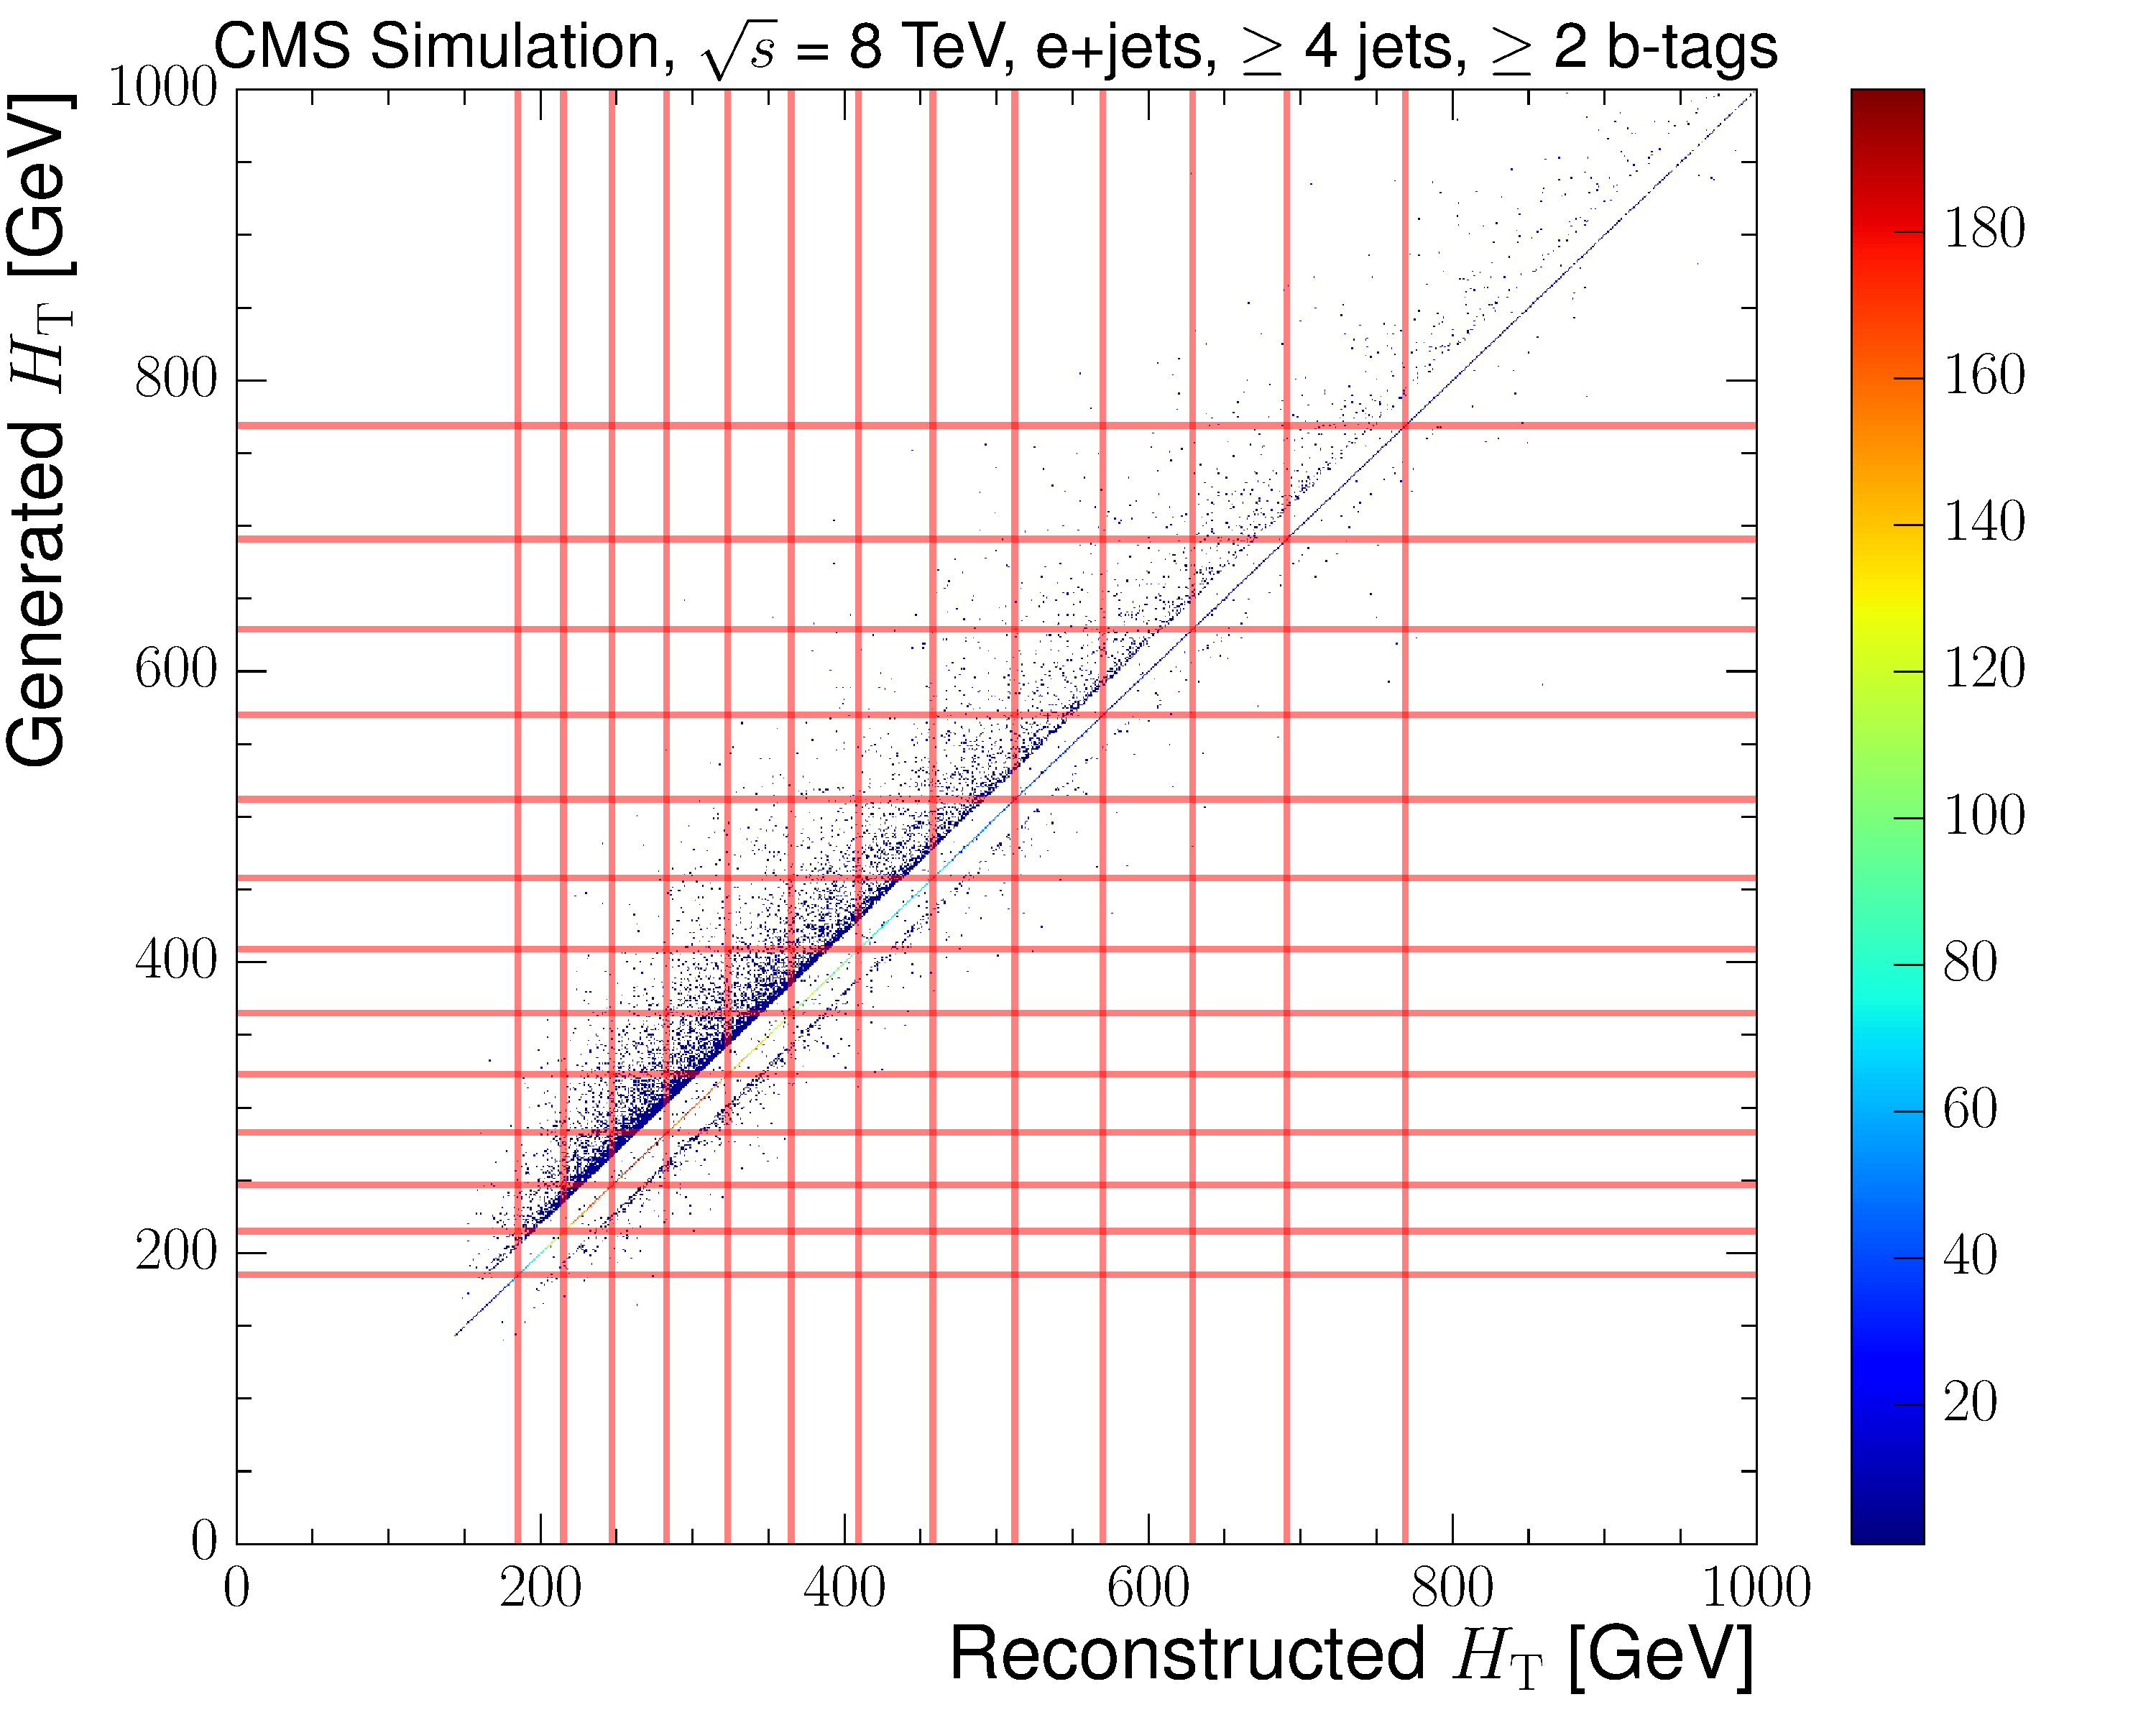
\includegraphics[width=0.48\textwidth]{Chapters/04_Analysis/04b_XSections/images/binning/electron_HT_8TeV.pdf}\\
     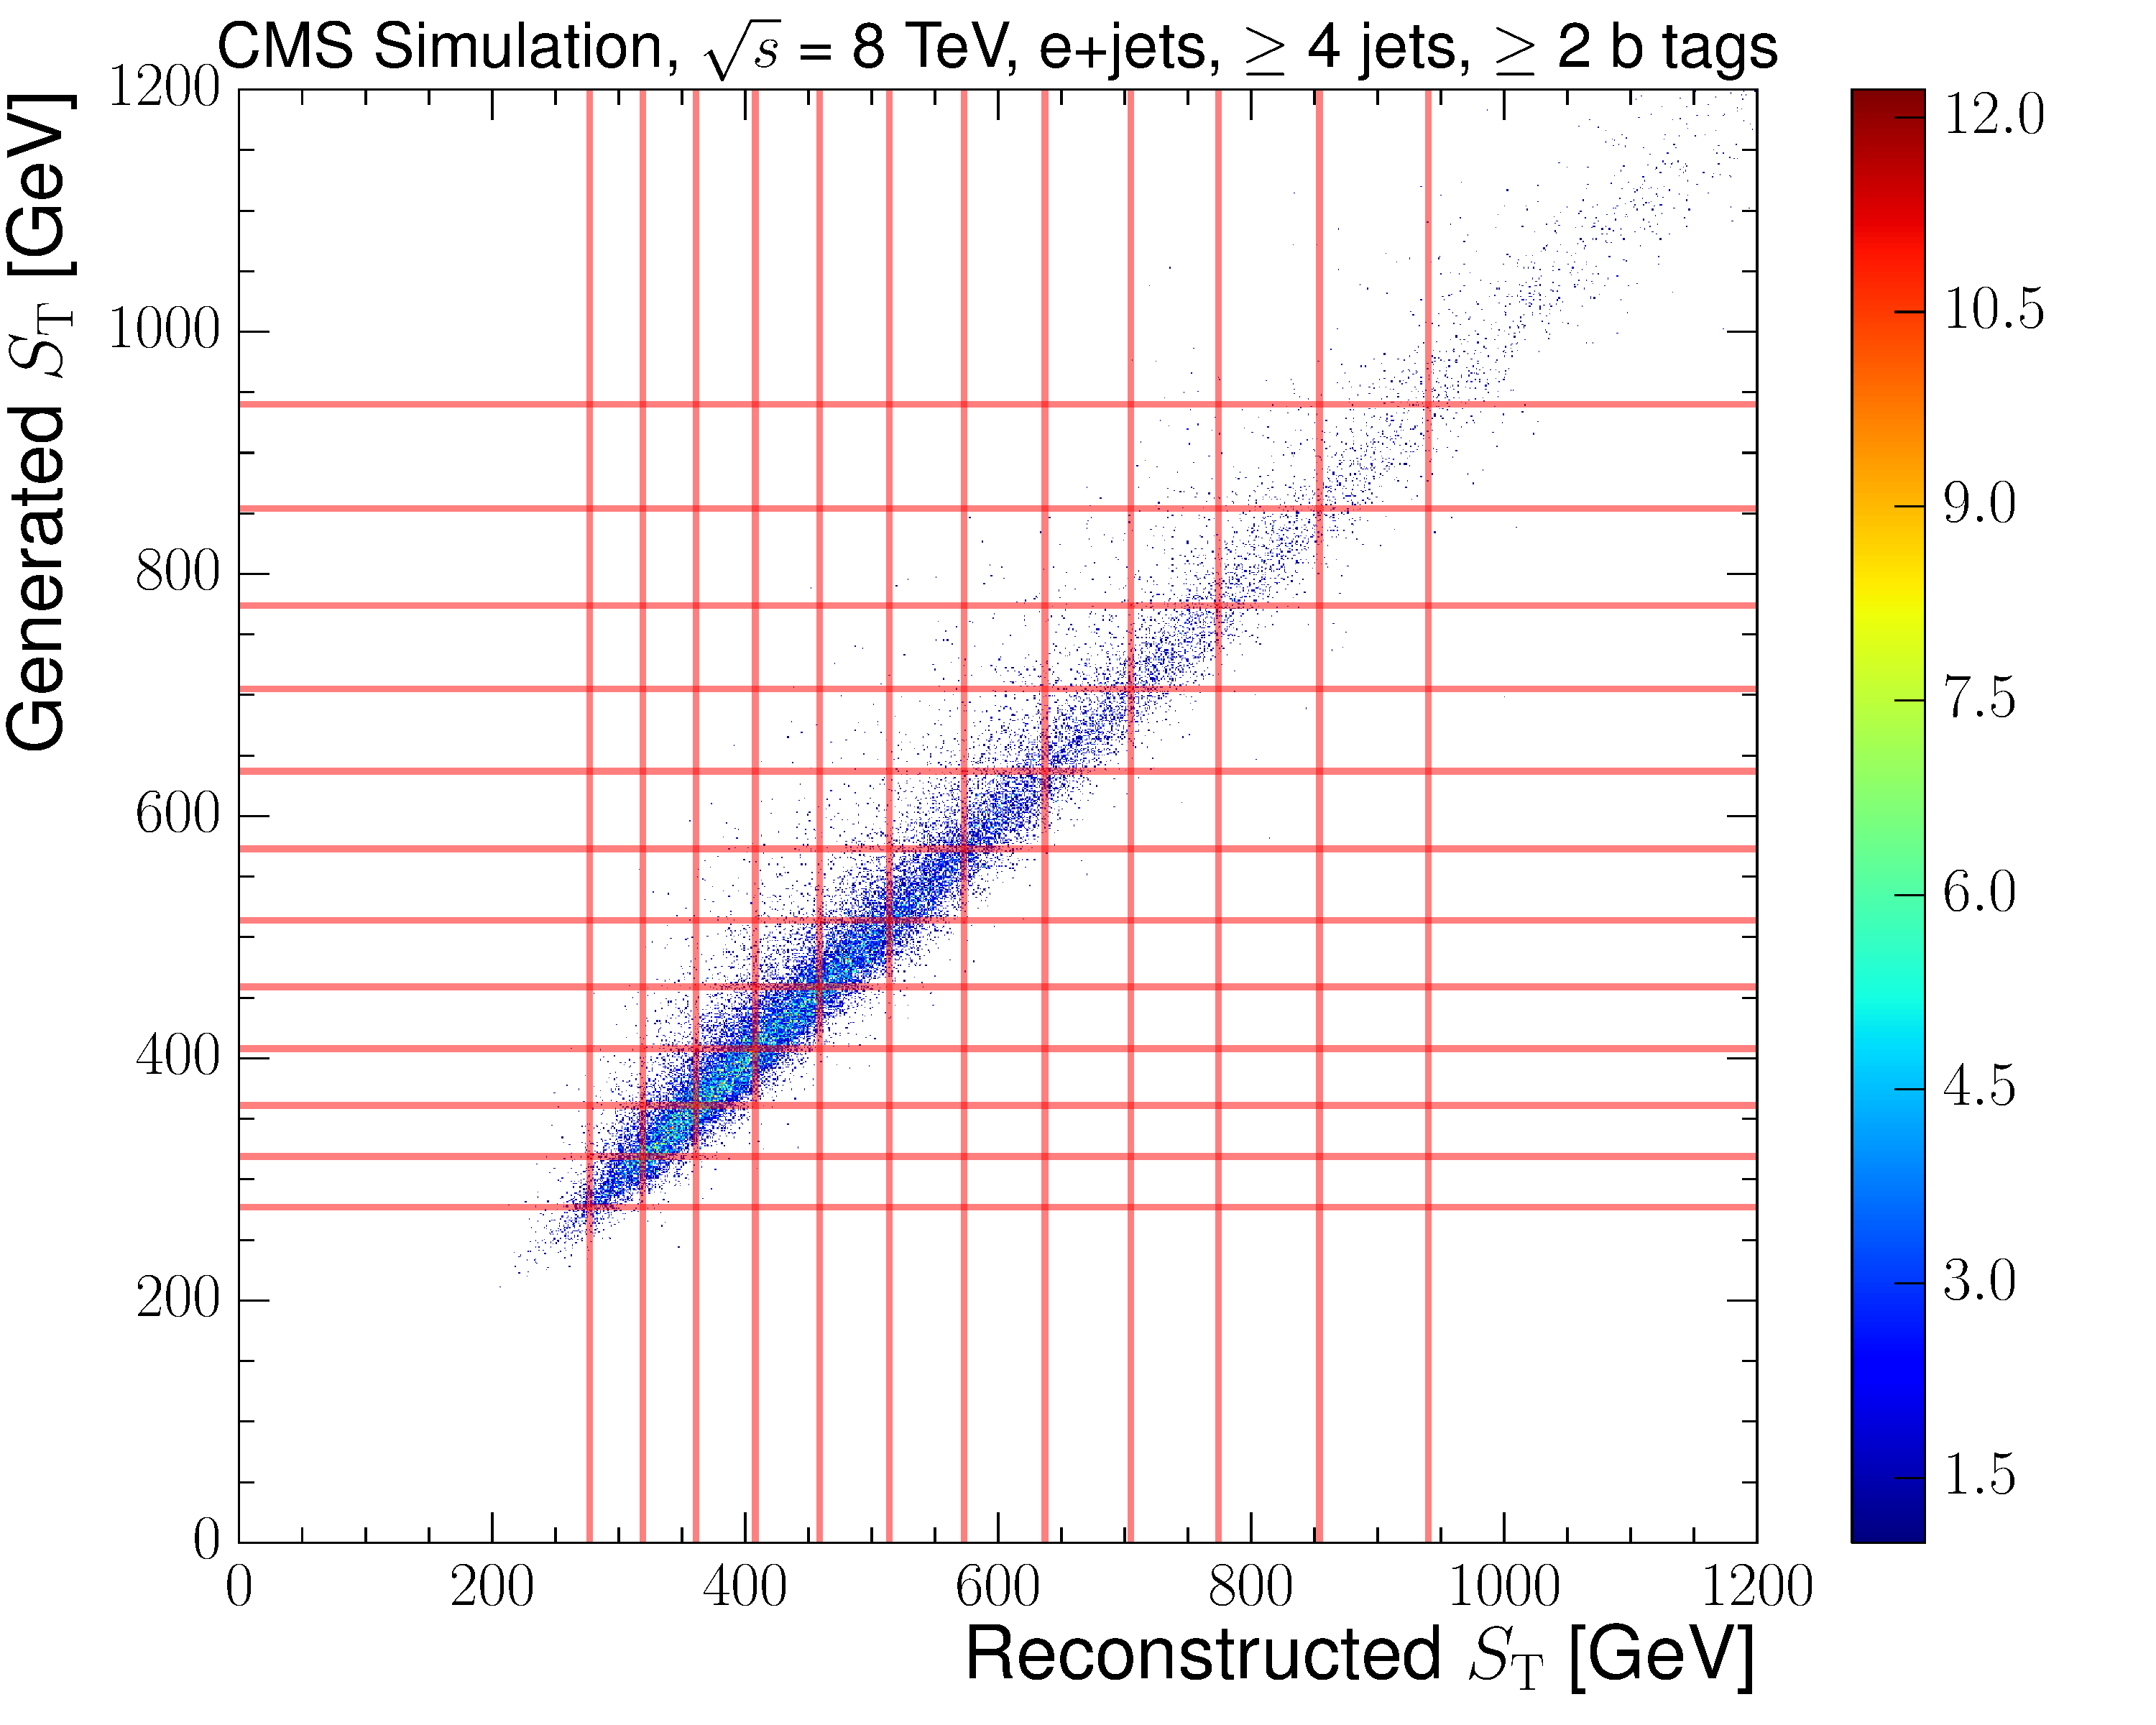
\includegraphics[width=0.48\textwidth]{Chapters/04_Analysis/04b_XSections/images/binning/electron_ST_8TeV.pdf}\hfill
     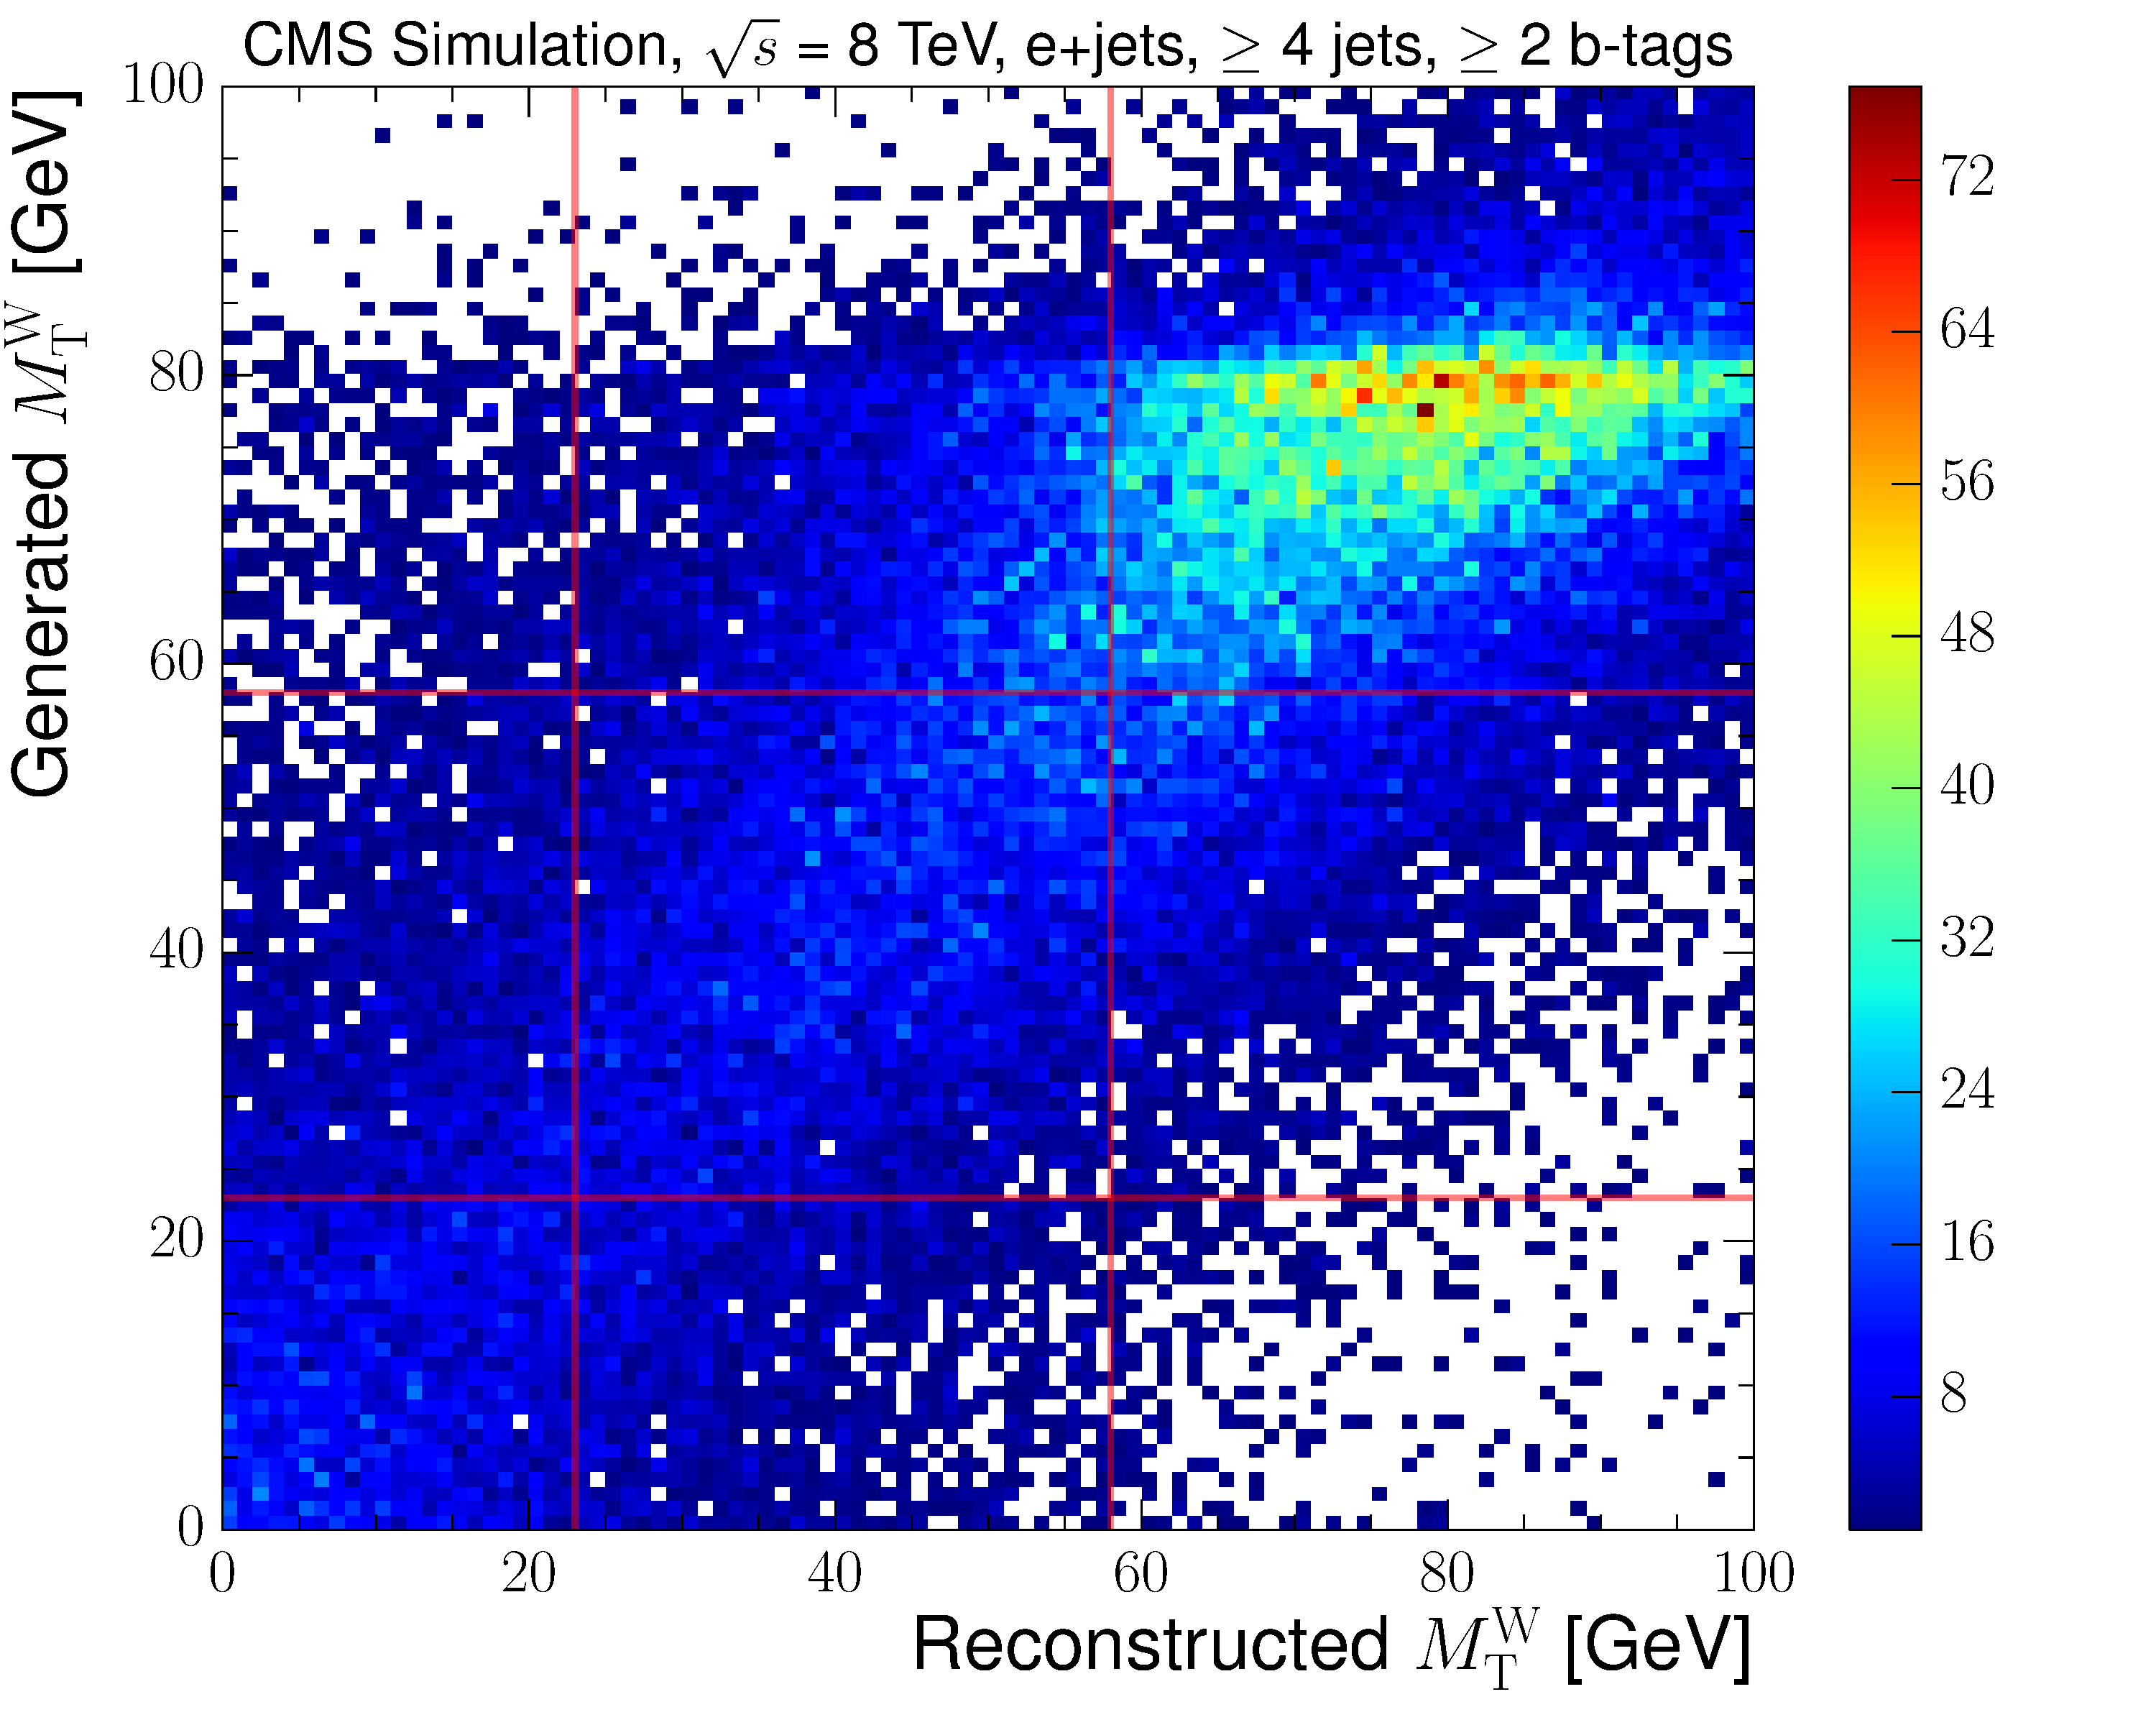
\includegraphics[width=0.48\textwidth]{Chapters/04_Analysis/04b_XSections/images/binning/electron_MT_8TeV.pdf}\\
	 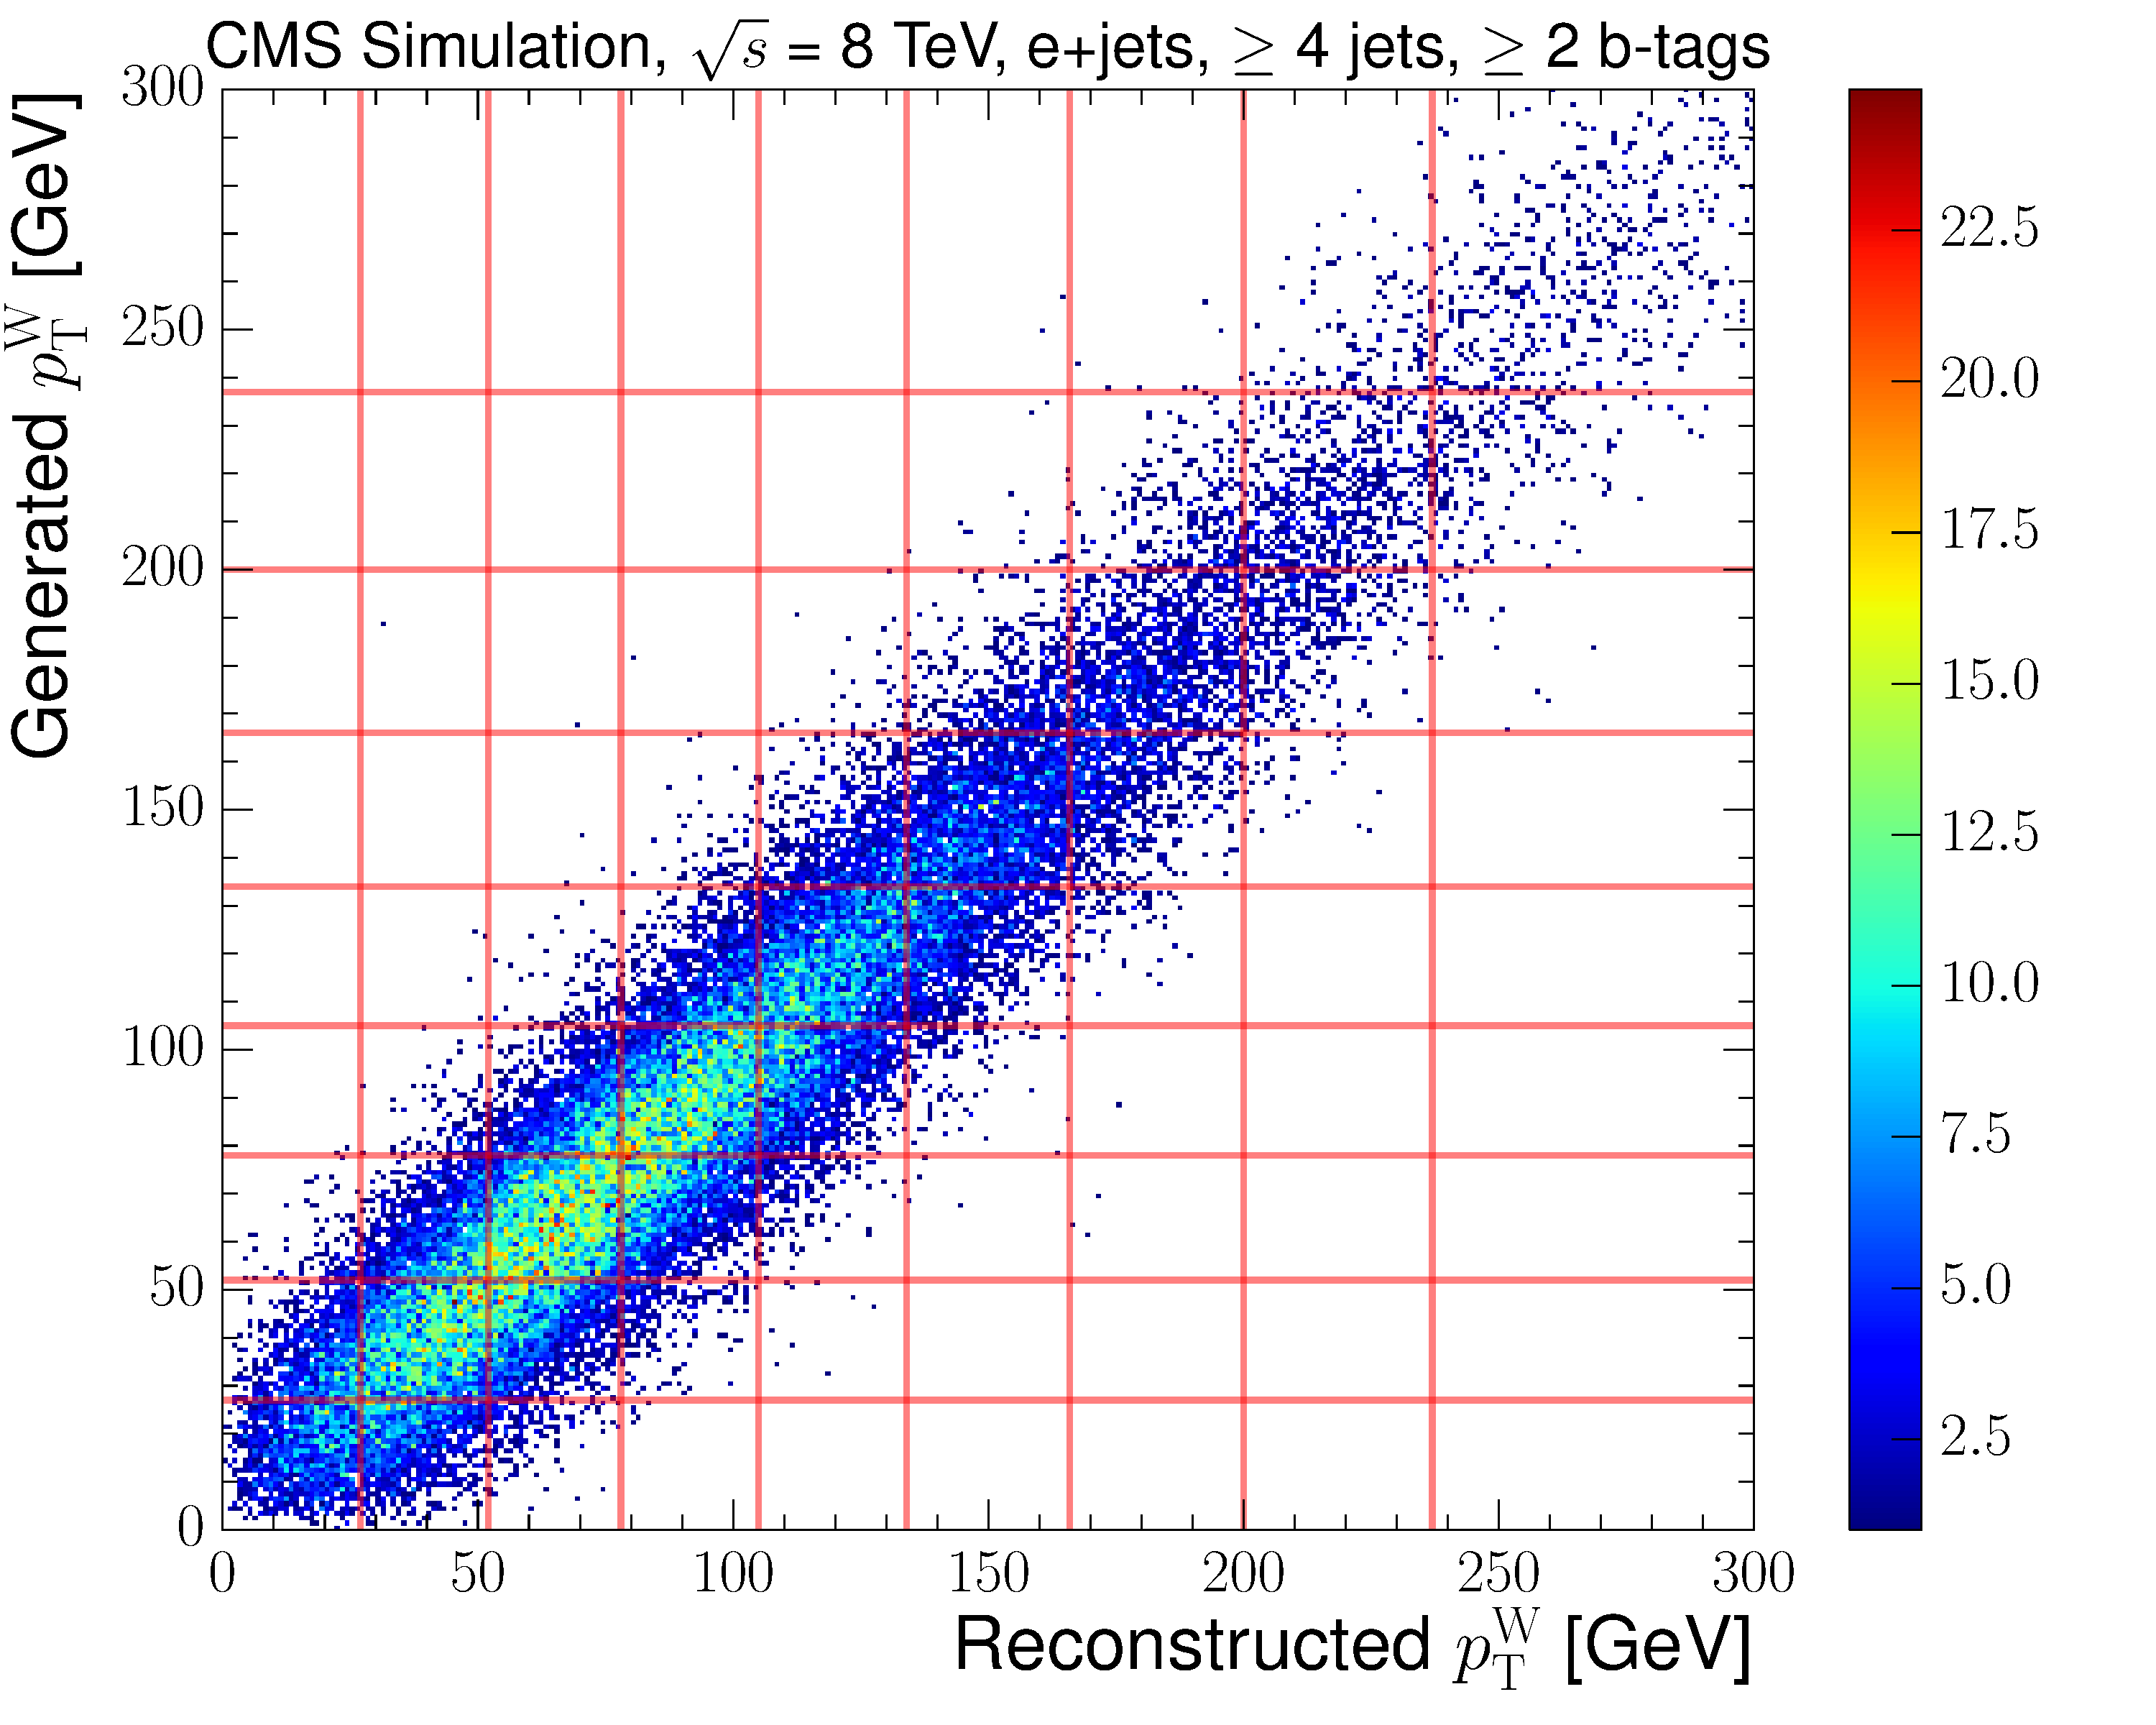
\includegraphics[width=0.48\textwidth]{Chapters/04_Analysis/04b_XSections/images/binning/electron_WPT_8TeV.pdf}\hfill
	 \caption{Generated versus reconstructed distributions of the primary variables \met (upper left), \HT (upper
	 right), \st (middle left), \mt (middle right) and \wpt (lower) with horizontal and vertical lines
	 representing the boundaries of the selected bins at $\sqrt{s}=8\TeV$ in the electron+ jets channel. These
	 distributions are obtained using \ttbar Monte Carlo simulation.}
     \label{fig:binning_8TeV_electron}
 \end{figure}

\section{Maximum Likelihood Fit}
\label{maximum_likelihood_fit}
A maximum log likelihood fit of four templates to data in each bin of the primary variables is used to obtain
the number of events in each bin. The four templates used are \ttbar, single top, V+Jets (a combination of
W+Jets and Z+Jets events) and QCD. The template distributions are obtained from the following three
variables: the absolute pseudorapidity of the lepton (\abseta), the three-dimensional angle between the lepton
and the nearest \bjet ($\alpha$), and the invariant mass of the three jets with the highest \pt sum ($M3$).

The fit is carried out by MINIMISING the negative log of the likelihood function (LL):

\begin{equation}
\label{log_likelihood}
LL\left(x_i, d_i\right) = -2 \log{\prod\limits_{i}\frac{x_i^{d_i}\cdot
e^{-x_i}}{d_i!}}=-2\sum\limits_{i}\log{\left(\frac{x_i^{d_i}\cdot e^{-x_i}}{d_i!}\right)}.
\end{equation}

where $i$ is the bin index in the template, $x_i$ is the total of all the templates in bin $i$, and $d_i$ is
the observed number of data events in  bin $i$.

Fitting using more than one fitting variable (the three aforementioned fitting variables), the log likelihoods
are summed:
\begin{equation}
\label{eq:log_L_final}
LL\left(x, d\right) = -\frac{2}{k} \sum\limits_{k} \log{L_k}
\end{equation}

where $L_k$ is the likelihood function of each of the different fit variables. Here the division by $k$
accounts for the fact that the same information is used in all three fit variables, and provides a
conservative estimate of the uncertainties in the resulting fitted parameters.

A simultaneous fit is done with three templates in bins of
each variable.
- V\_Jets template combined over all global variable bins.
- QCD template also inclusive over all global variable bins



\subsection{Choice of templates}
\label{choice_of_templates}

Three fitting variables are used because no individual fit variable is able to distinguish between all four
templates used in the fit:

\begin{itemize}
  \item {\ttbar}
  \item{single-top}
  \item{V+jets (W+jets + Z+jets}
  \item{QCD multi-jet} 
\end{itemize}

\ttbar, single-top and V+jets templates are taken from simulation, while the QCD template is extracted from
datas described in Section~\ref{ss:background_selection}. These four template shapes in each of the three
fitting variables are shown in Figures~\ref{fig:fit_variable_distributions_7TeV} and
\ref{fig:fit_variable_distributions_8TeV} for $\sqrt{s}=7\TeV$ and $\sqrt{s}=8\TeV$ respectively. The fit
variables all show reasonable distinction between the templates. Single top events have similar signatures to
\ttbar events, with a central lepton from the decay of the single top, leading to a single top template that
is similar to the \ttbar template in the electron \abseta and muon \abseta distributions. In the $\alpha$
distribution, the similarity is attributable to the fact that the average boost for single top events is lower
than in \ttbar events, leading to a wider single top template. The M3 variable will be a combination of the
jets from the hadronically decaying \tquark (a \bjet and two other jets from the \W-boson) in \ttbar events,
wheras in the other templates, M3 will simply correspond to some random combination of jets in the event.
Hence, M3 shows the best discrimination between the single top and \ttbar templates.

\begin{figure}[hbtp]
    \centering
     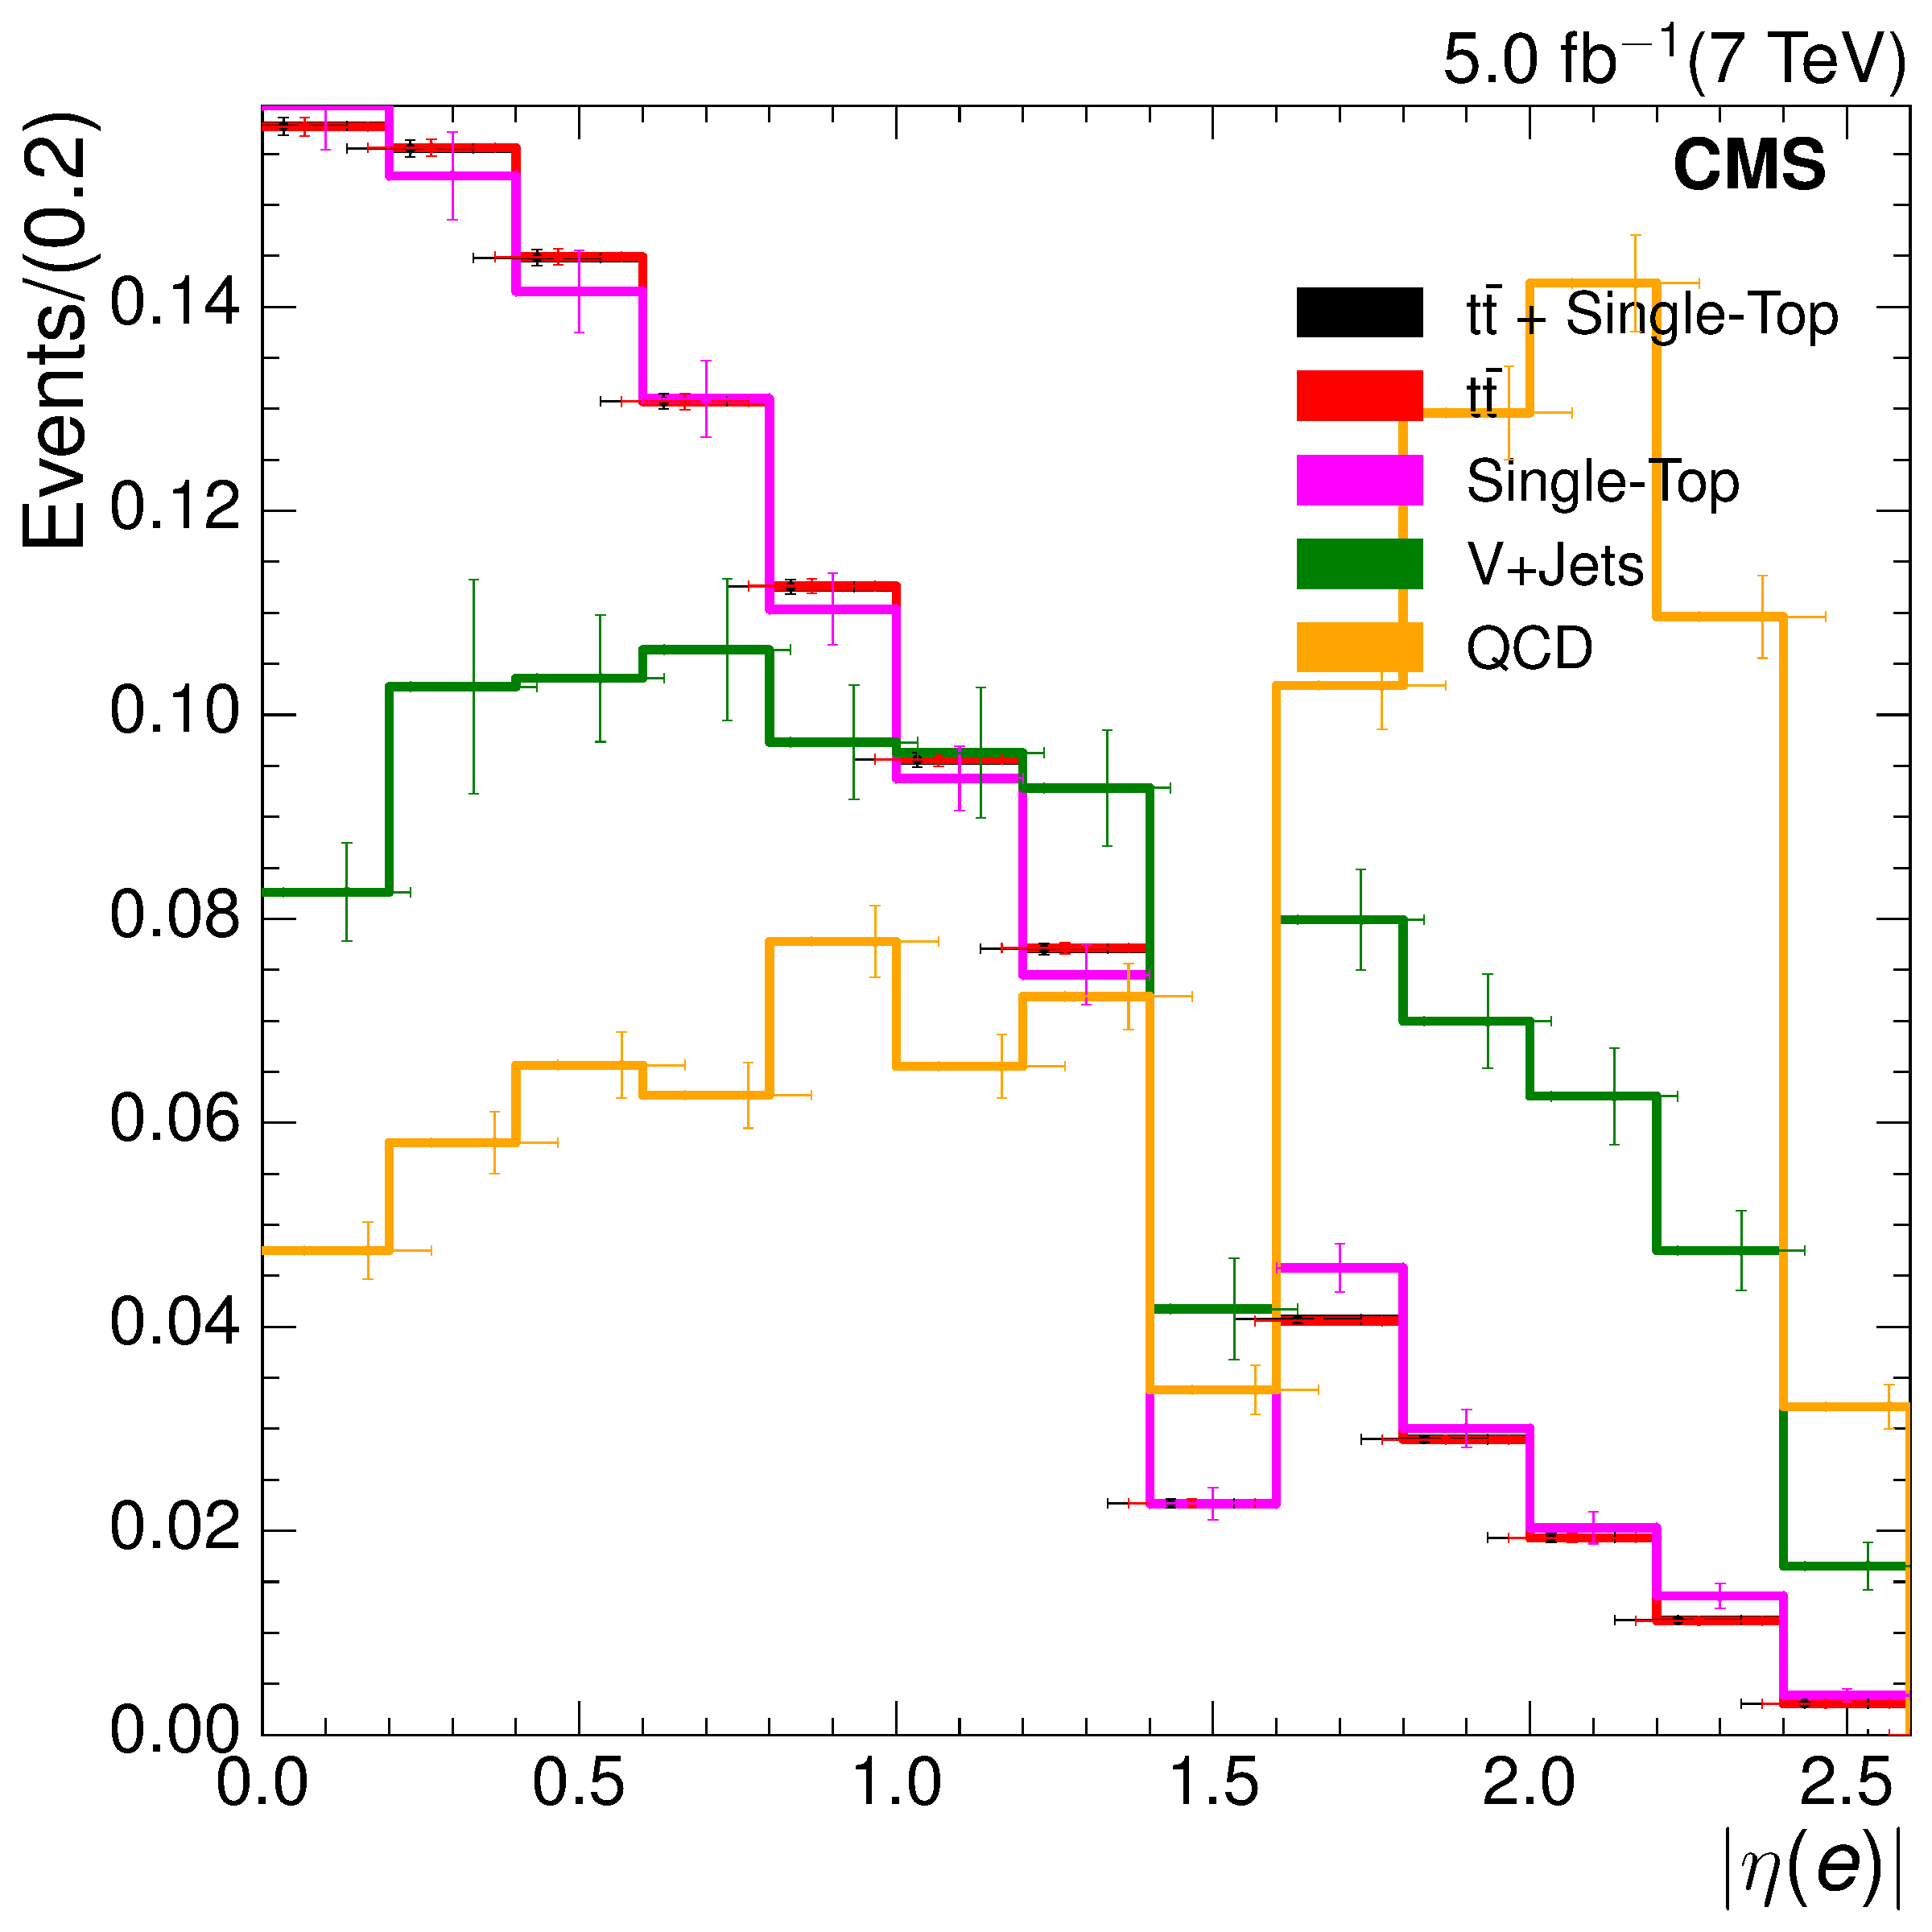
\includegraphics[width=0.48\textwidth]{Chapters/04_Analysis/04b_XSections/images/7TeV/fit_variables/MET/electron_absolute_eta/MET_inclusive_electron_absolute_eta_2orMoreBtags_templates.pdf}\hfill
     
\includegraphics[width=0.48\textwidth]{Chapters/04_Analysis/04b_XSections/images/placeholder.png}\\
     %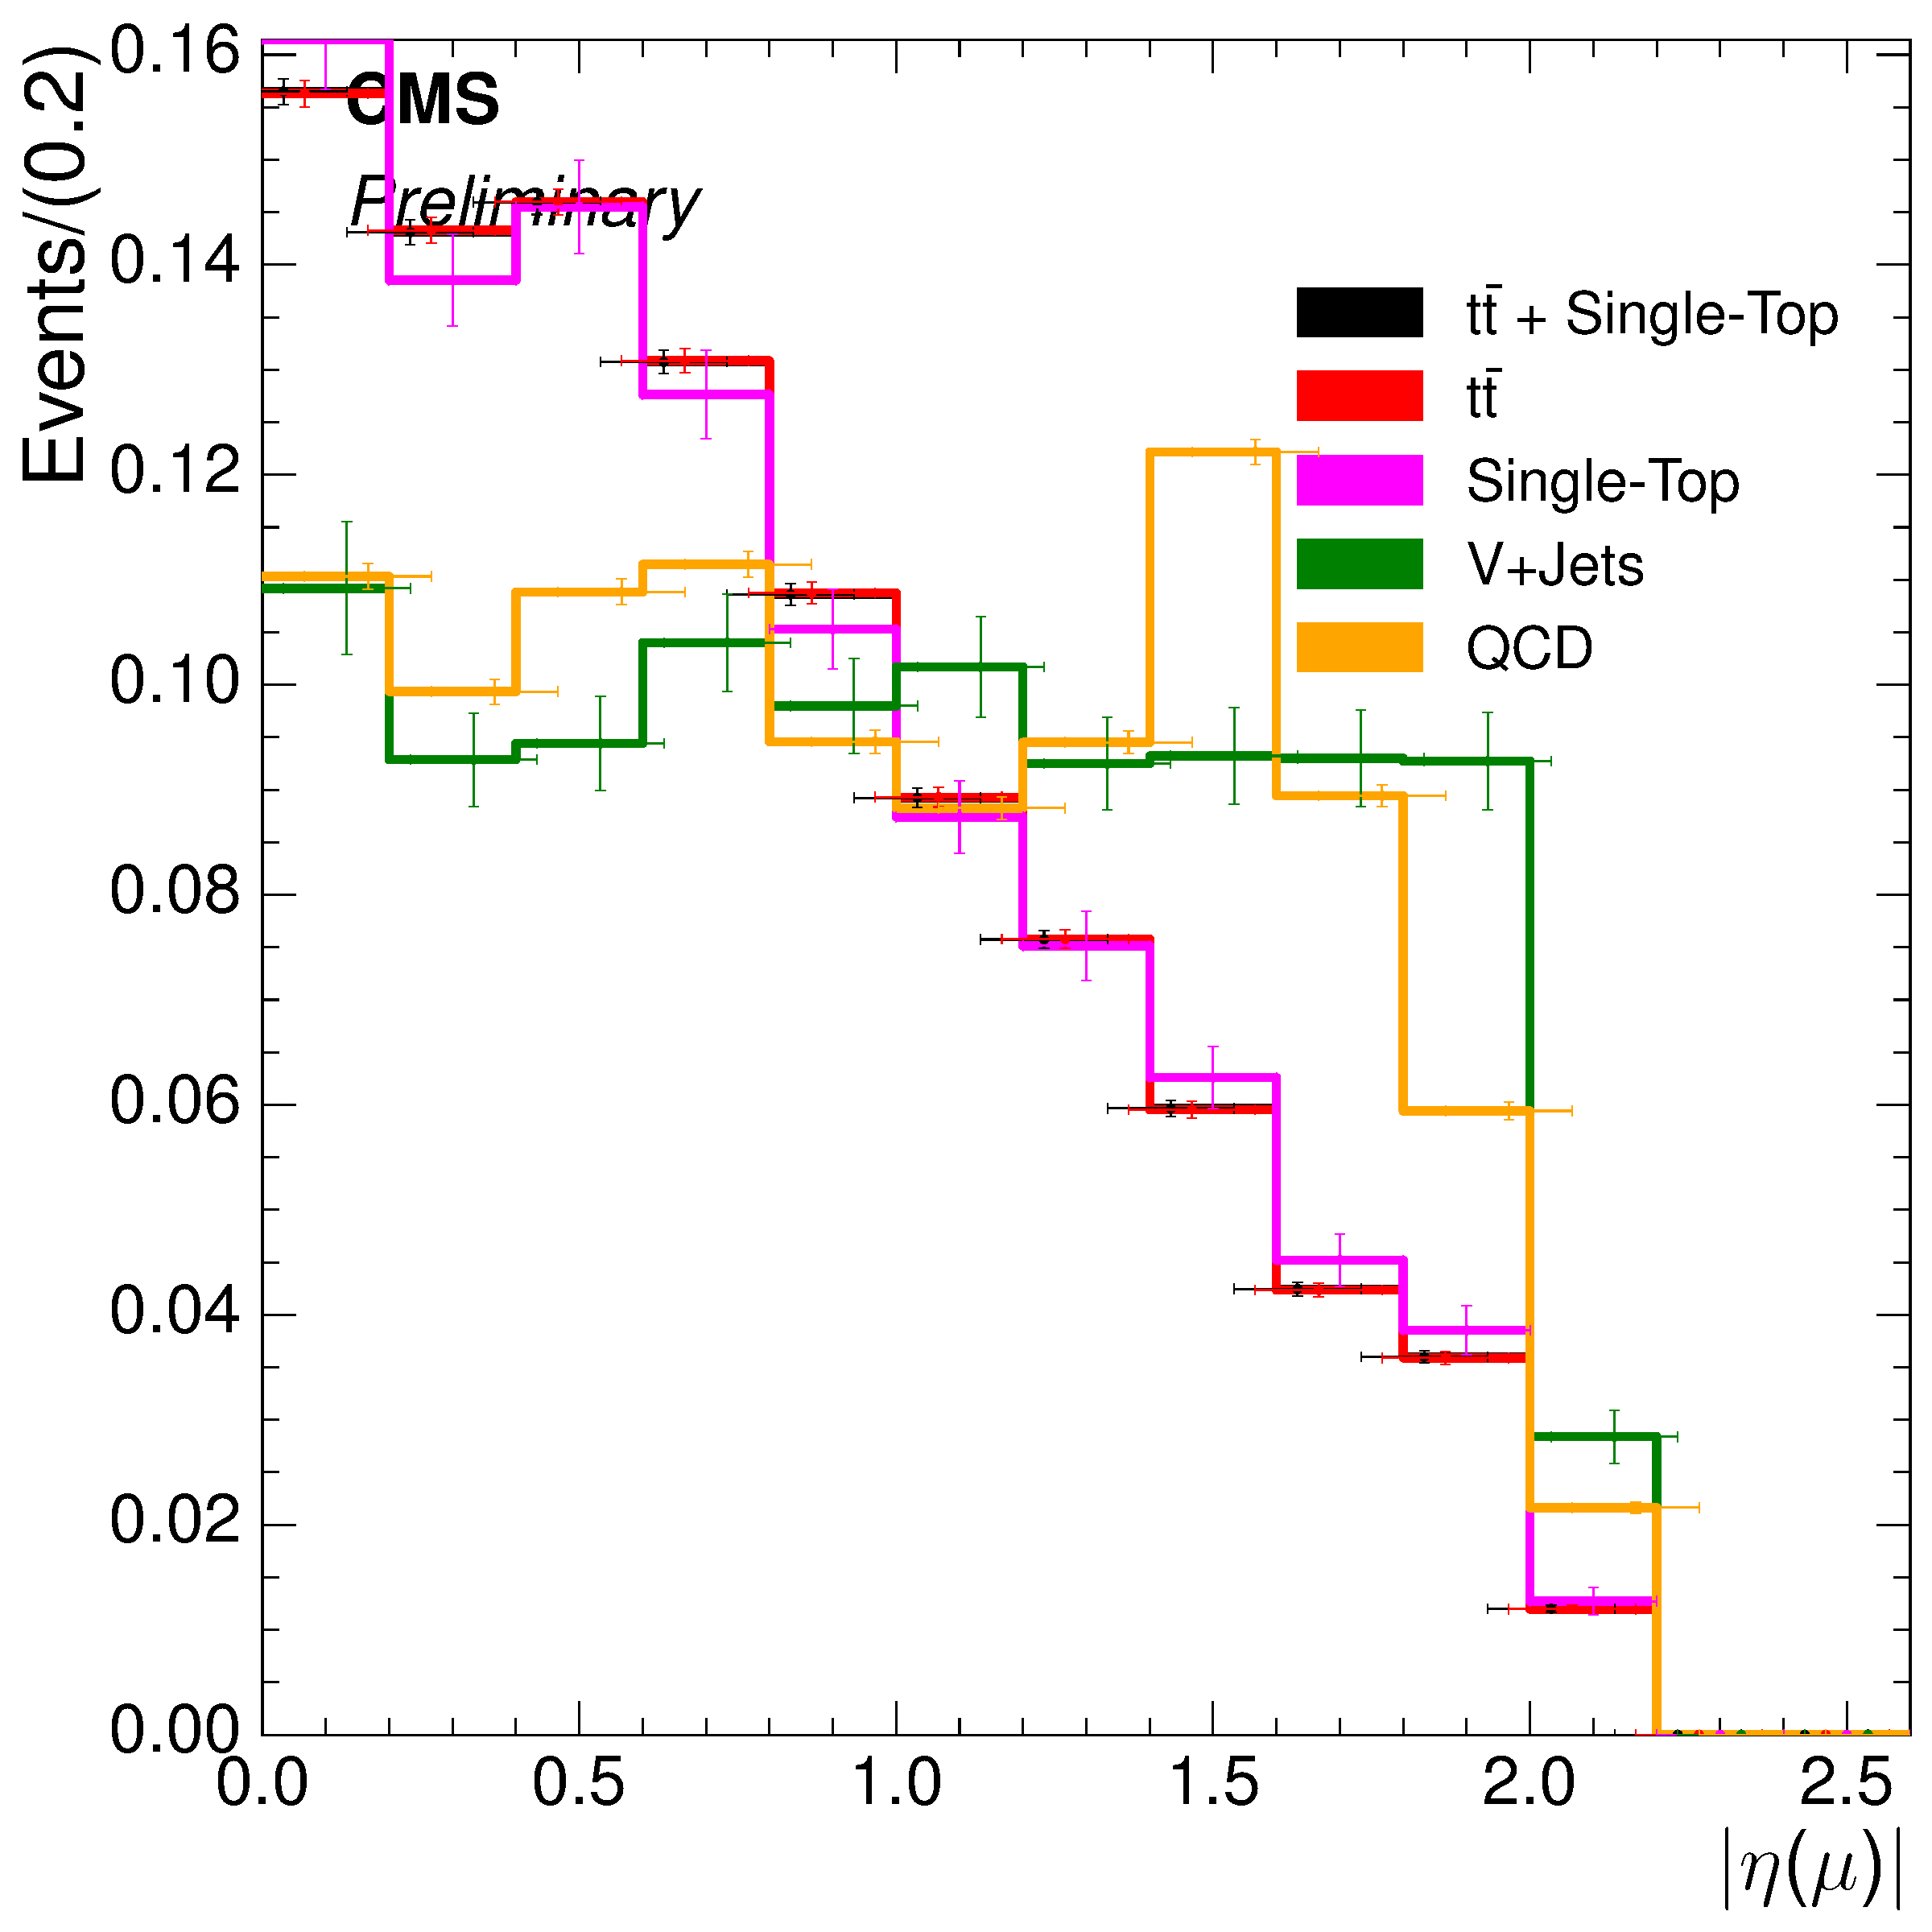
\includegraphics[width=0.48\textwidth]{Chapters/04_Analysis/04b_XSections/images/7TeV/fit_variables/MET/muon_absolute_eta/MET_inclusive_muon_absolute_eta_2orMoreBtags_templates.pdf}\\    
     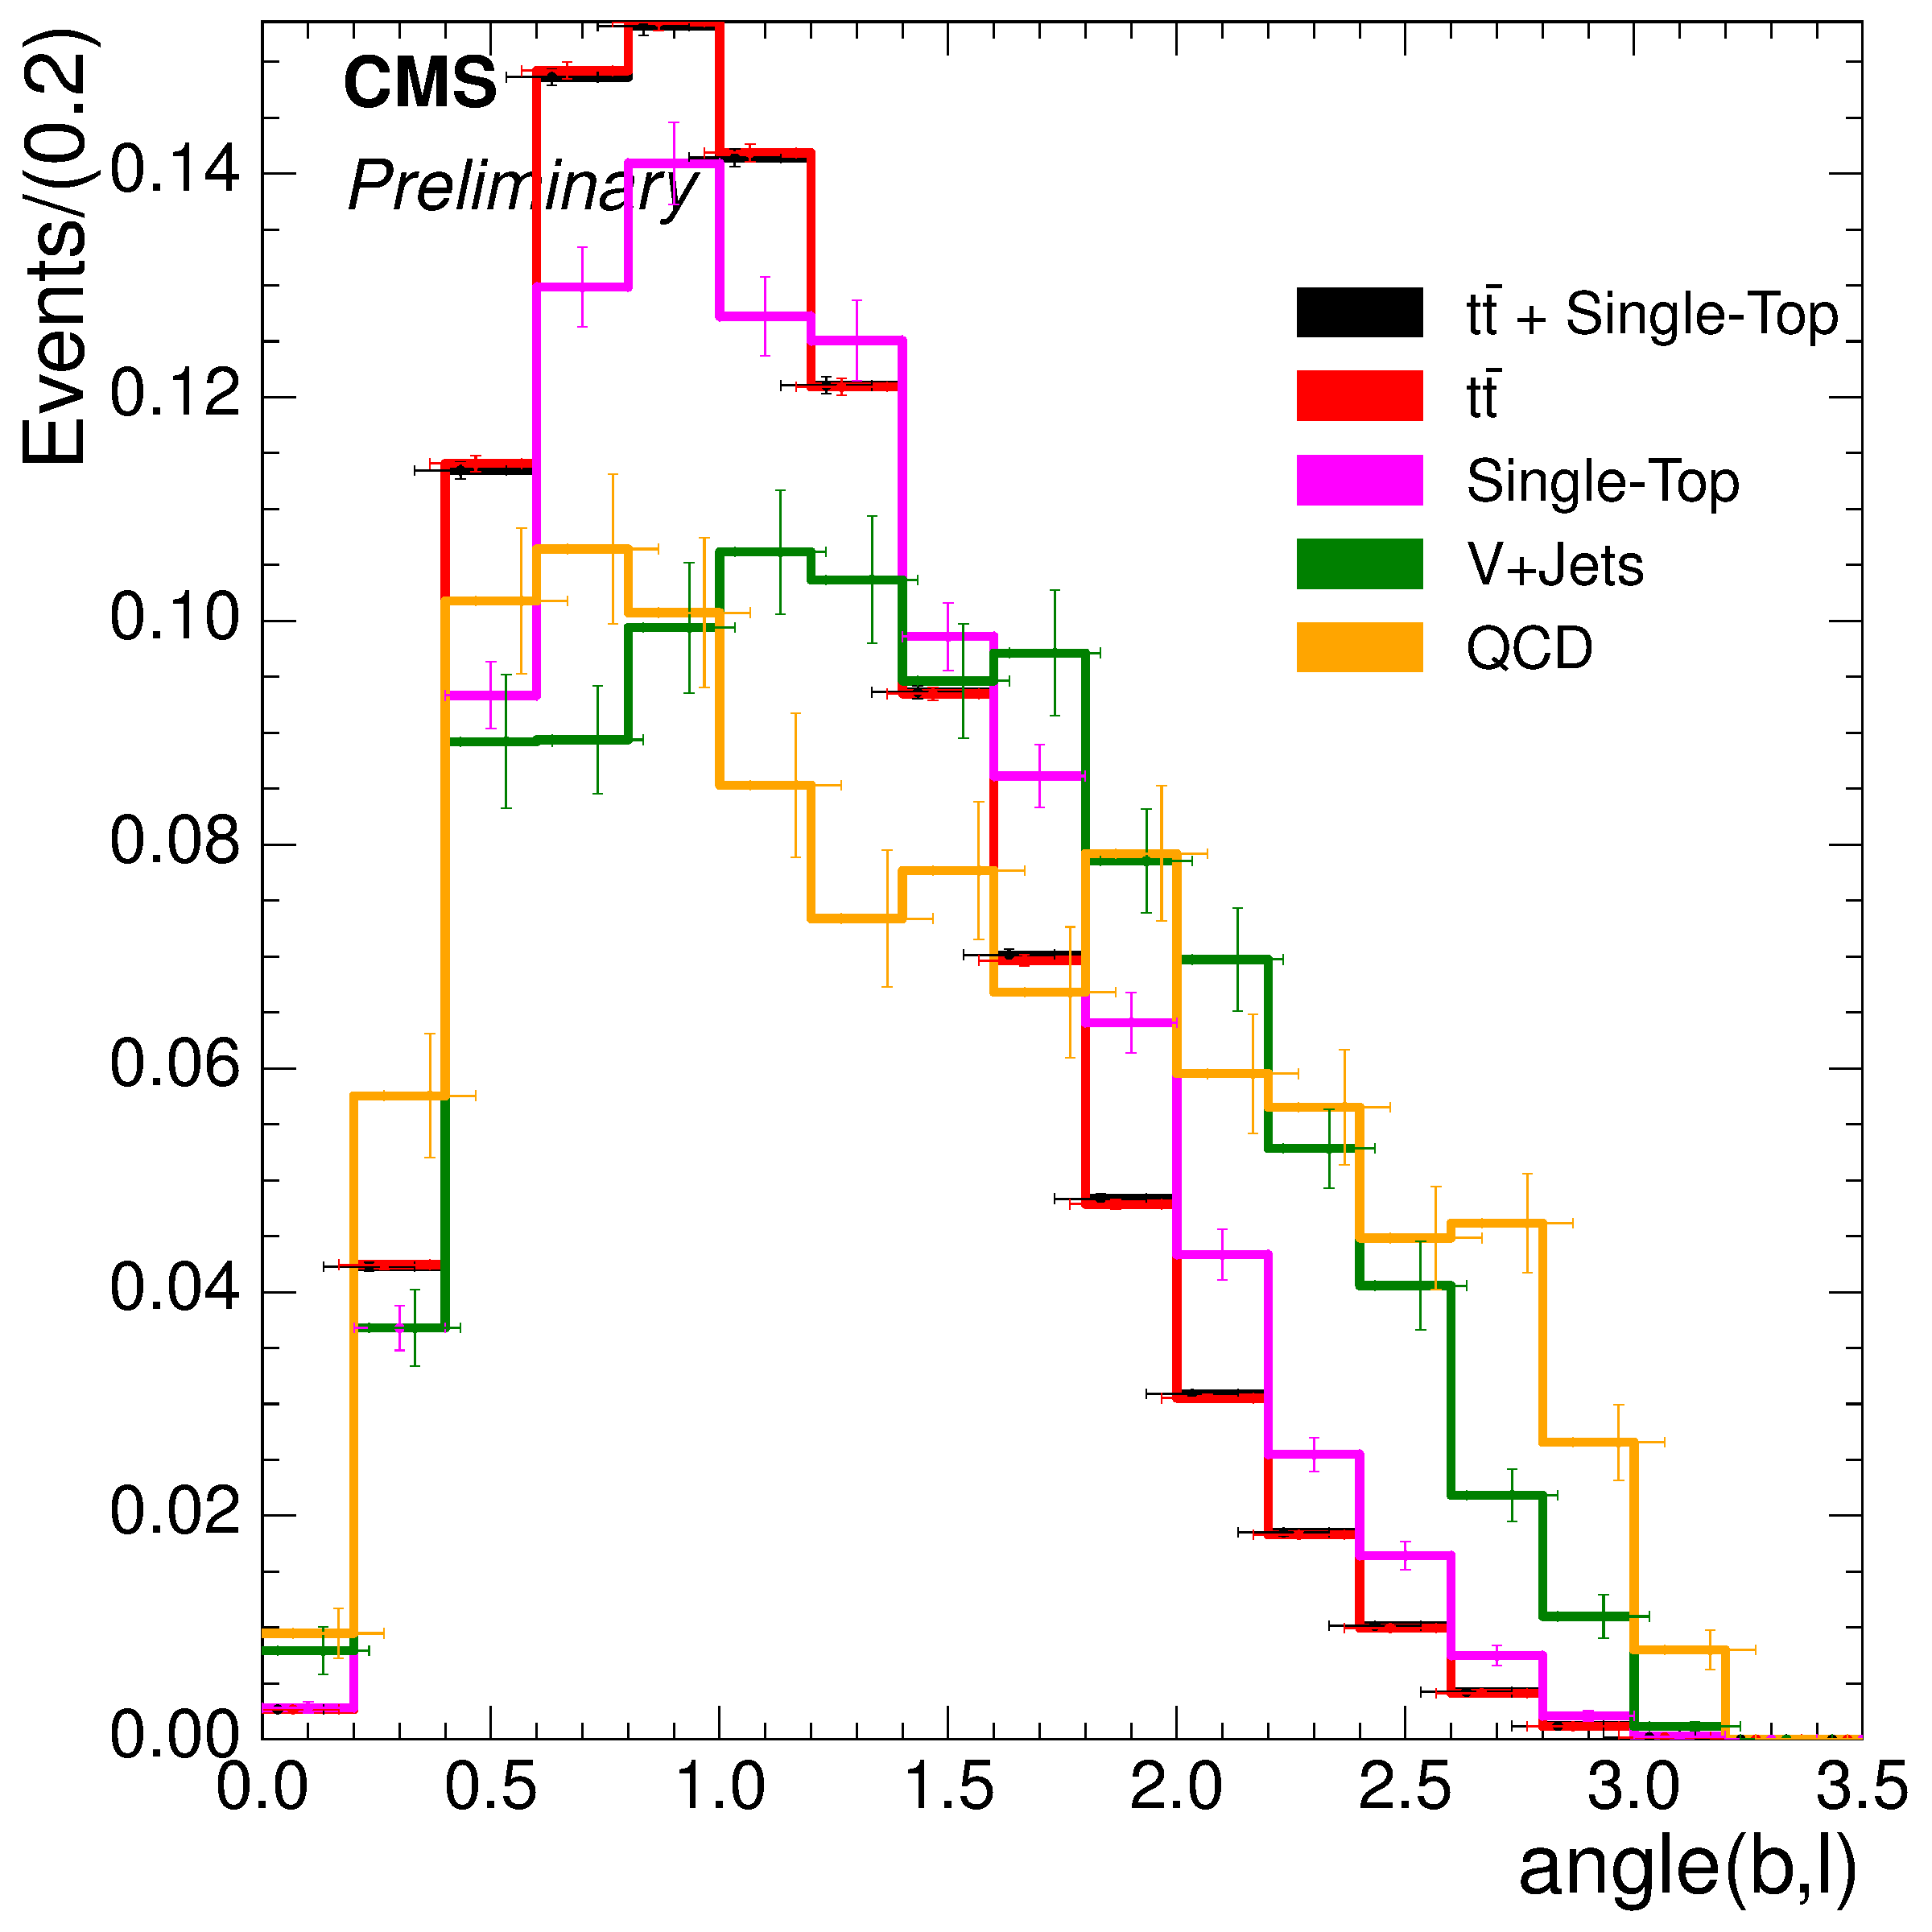
\includegraphics[width=0.48\textwidth]{Chapters/04_Analysis/04b_XSections/images/7TeV/fit_variables/MET/angle_bl/MET_inclusive_angle_bl_2orMoreBtags_templates.pdf}\hfill
     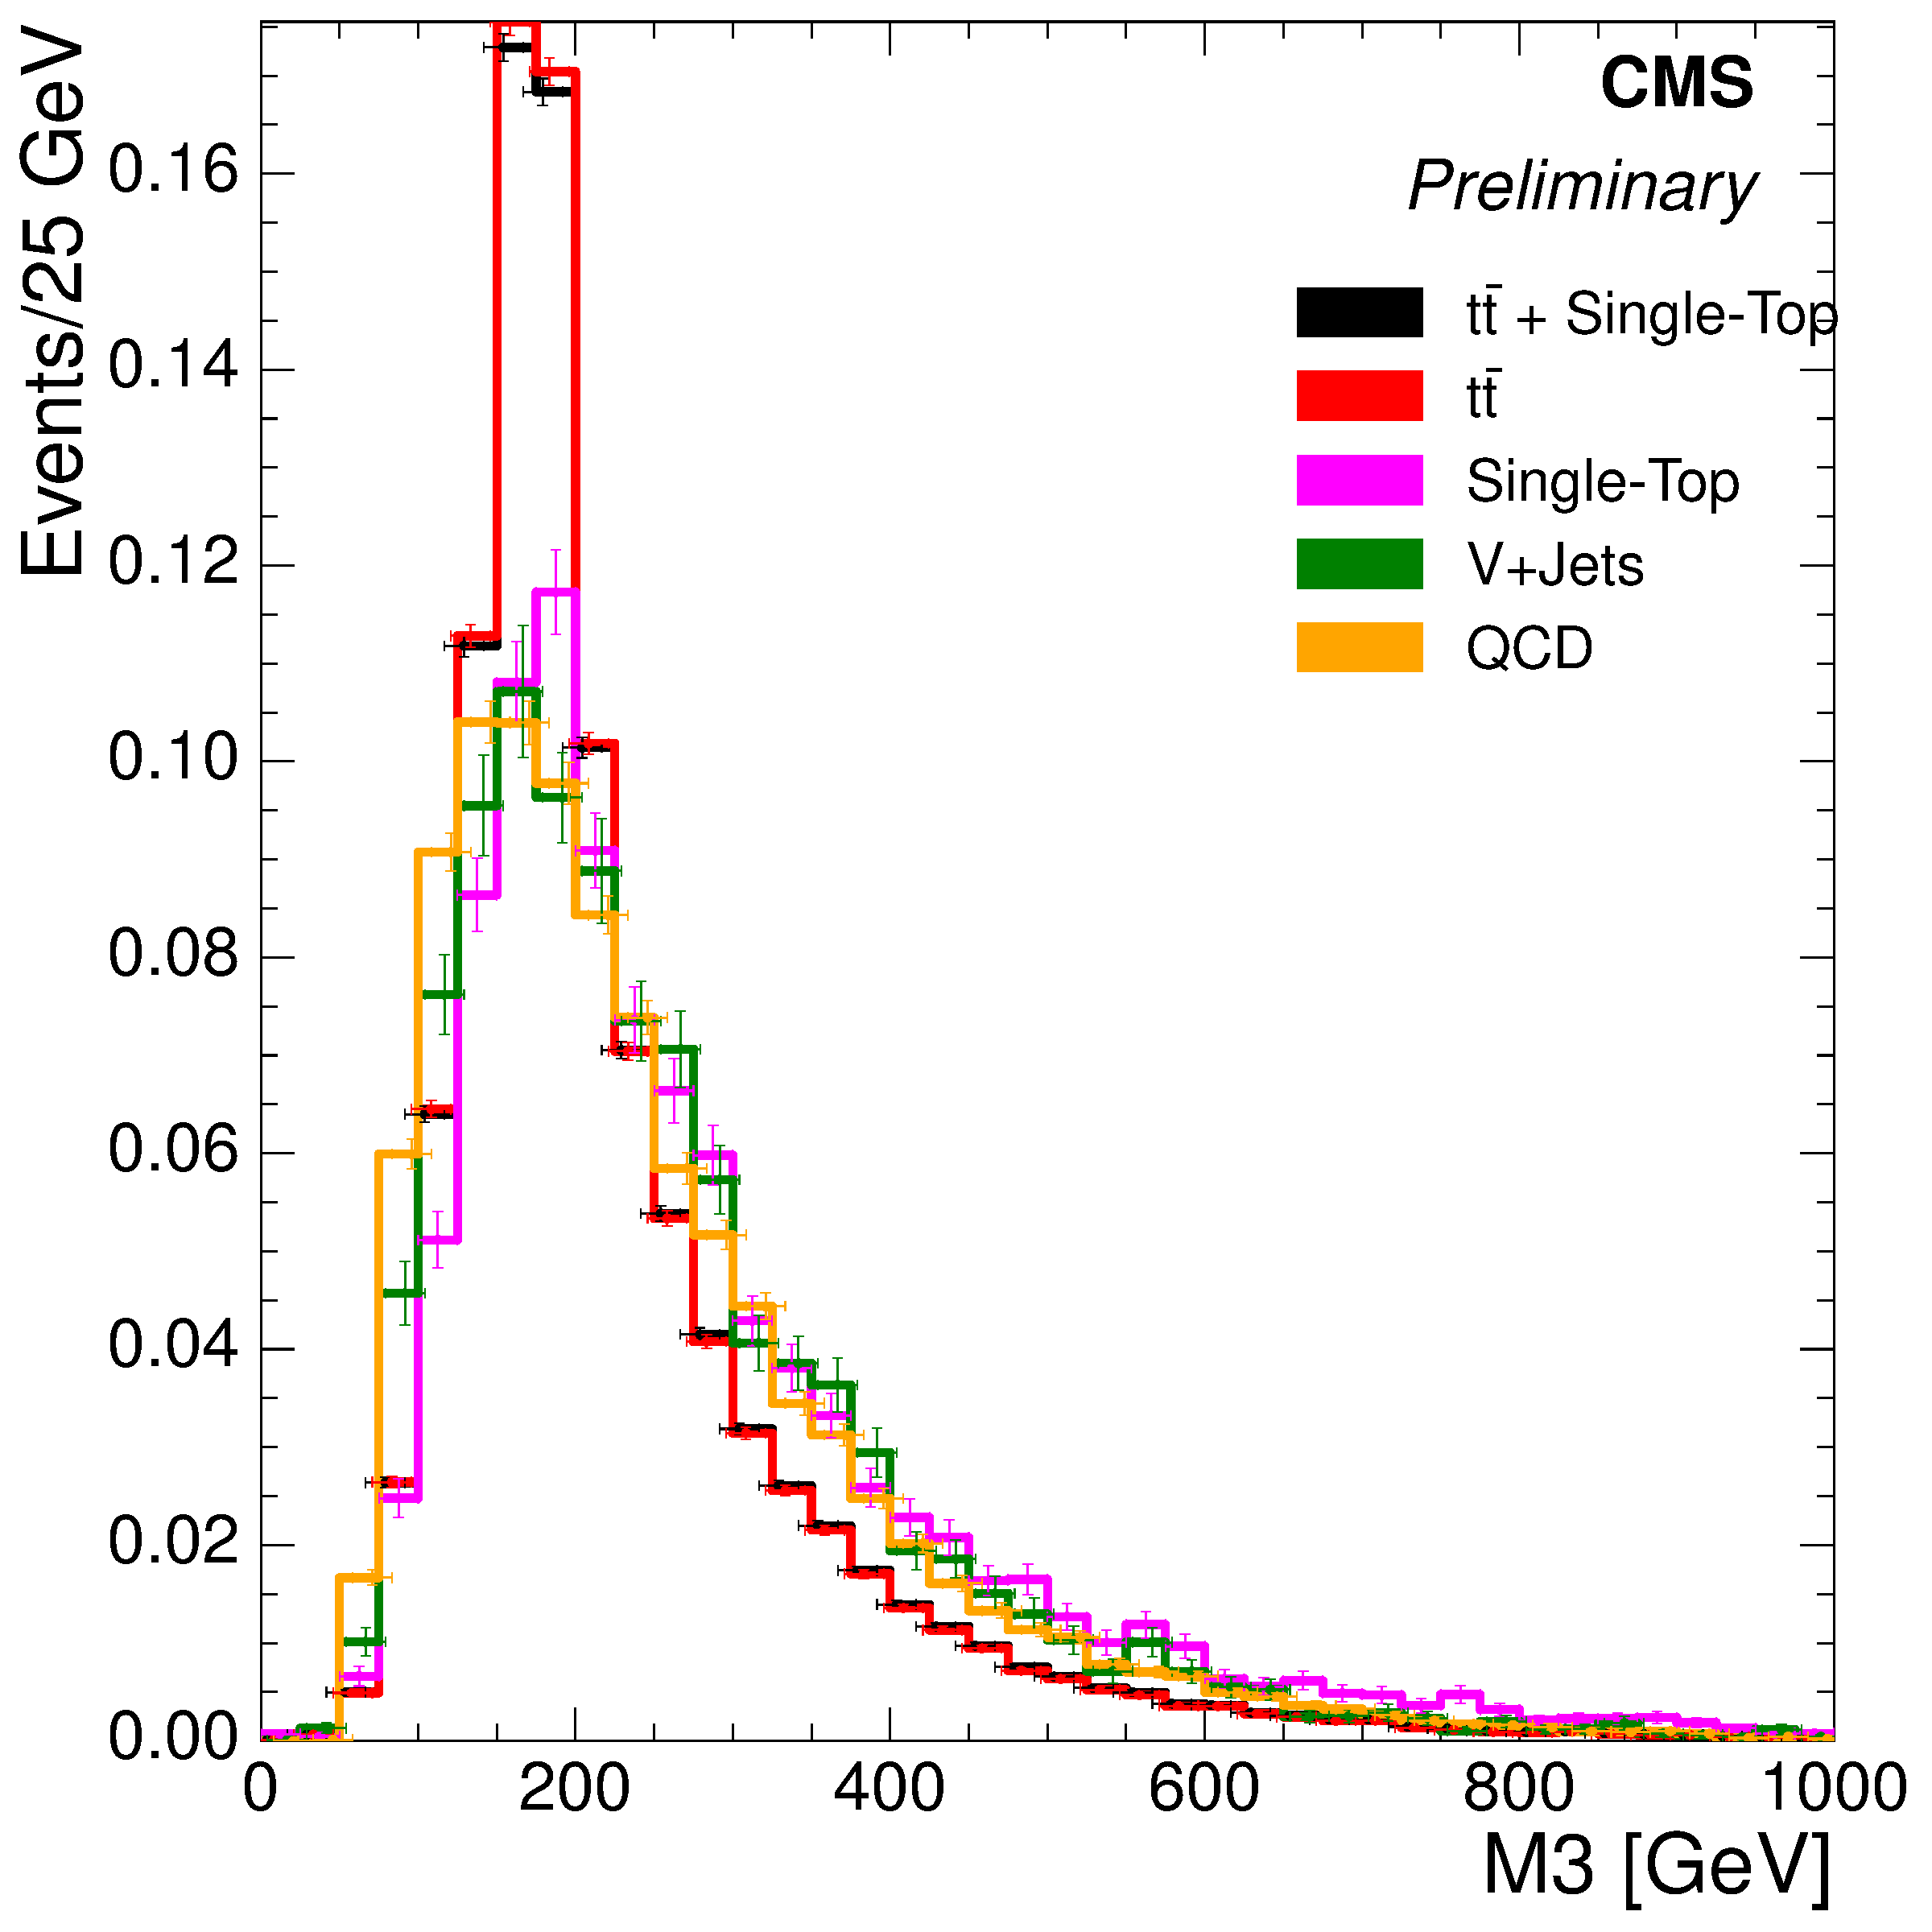
\includegraphics[width=0.48\textwidth]{Chapters/04_Analysis/04b_XSections/images/7TeV/fit_variables/MET/M3/MET_inclusive_M3_2orMoreBtags_templates.pdf}\\
	 \caption{Normalised distributions of the four templates for the three fit variables at $\sqrt{s}=7\TeV$,
	 inclusive across all primary variable bins: electron \abseta (upper left), muon \abseta (upper right),
	 $\alpha$ (lower left) and M3 (lower right).}
     \label{fig:fit_variable_distributions_7TeV}
\end{figure}

\begin{figure}[hbtp]
    \centering
     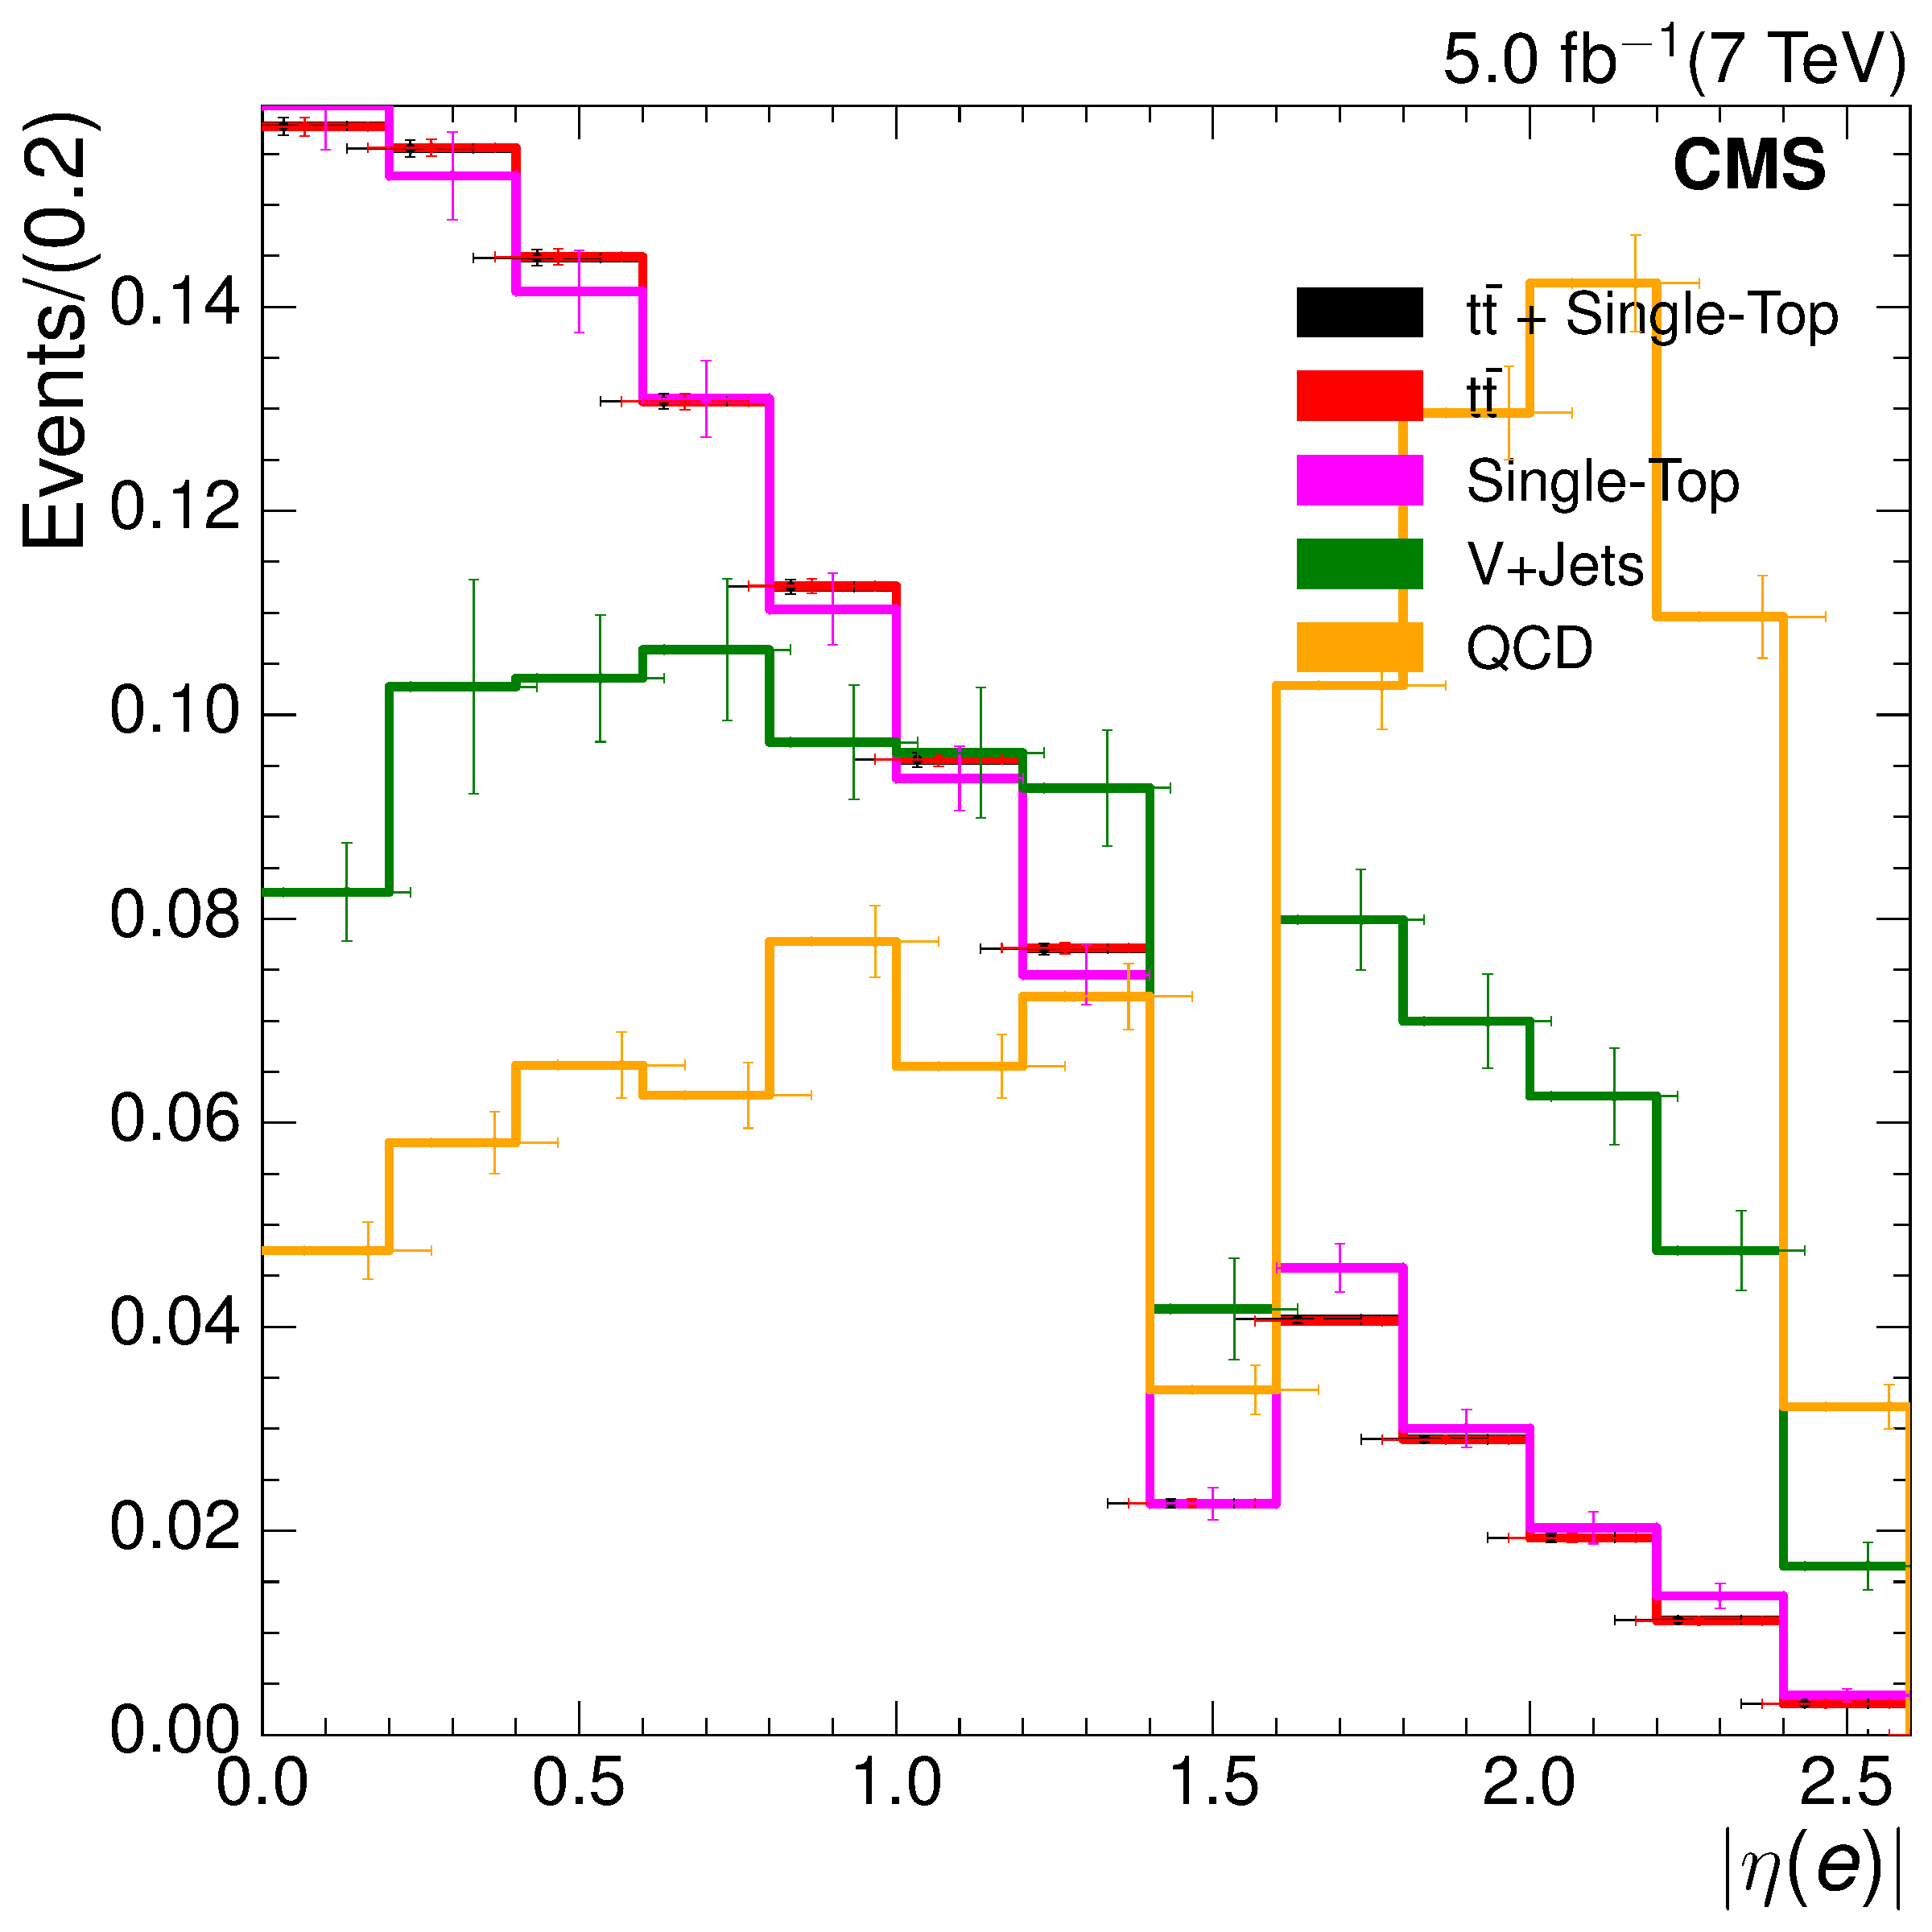
\includegraphics[width=0.48\textwidth]{Chapters/04_Analysis/04b_XSections/images/7TeV/fit_variables/MET/electron_absolute_eta/MET_inclusive_electron_absolute_eta_2orMoreBtags_templates.pdf}\hfill
     
\includegraphics[width=0.48\textwidth]{Chapters/04_Analysis/04b_XSections/images/placeholder.png}\hfill
     %\includegraphics[width=0.48\textwidth]{Chapters/04_Analysis/04b_XSections/images/7TeV/fit_variables/MET/muon_absolute_eta/MET_inclusive_muon_absolute_eta_2orMoreBtags_templates.pdf}\\    
     \includegraphics[width=0.48\textwidth]{Chapters/04_Analysis/04b_XSections/images/7TeV/fit_variables/MET/angle_bl/MET_inclusive_angle_bl_2orMoreBtags_templates.pdf}\hfill
     \includegraphics[width=0.48\textwidth]{Chapters/04_Analysis/04b_XSections/images/7TeV/fit_variables/MET/M3/MET_inclusive_M3_2orMoreBtags_templates.pdf}\\
	 \caption{Normalised distributions of the four templates for the three fit variables at $\sqrt{s}=7\TeV$,
	 inclusive across all primary variable bins: electron \abseta (upper left), muon \abseta (upper right),
	 $\alpha$ (lower left) and M3 (lower right).}
     \label{fig:fit_variable_distributions_8TeV}
\end{figure}

The QCD templates used are inclusive across all bins of the primary variables because there are low statistics
in the QCD background selection in higher bins. Figure~\ref{fig:fit_variable_qcd_comparisons_8TeV} shows the
a comparison between QCD templates in the lowest three bins of the \met variable and also the inclusive \met
QCD template. It can be seen that the third \met bin already shows low numbers of events, meaning the
inclusive template is largely shaped by events in the first two bins. Therefore, the inclusive QCD
background template is used rather than individual bins. Similar plots demonstrating the same behaviour for
the other primary variables are shown in Appendix~\ref{as:fitting_variable_QCD_template_comparisons}.

\begin{figure}[hbtp]
    \centering
     \includegraphics[width=0.48\textwidth]{Chapters/04_Analysis/04b_XSections/images/8TeV/fit_variables/MET/electron_absolute_eta/qcd/MET_electron_absolute_eta_0orMoreBtag_QCD_template_comparison.pdf}\hfill
     \includegraphics[width=0.48\textwidth]{Chapters/04_Analysis/04b_XSections/images/placeholder.png}\hfill
     %\includegraphics[width=0.48\textwidth]{Chapters/04_Analysis/04b_XSections/images/7TeV/fit_variables/MET/muon_absolute_eta/qcd/MET_inclusive_muon_absolute_eta_2orMoreBtags_templates.pdf}\\    
     \includegraphics[width=0.48\textwidth]{Chapters/04_Analysis/04b_XSections/images/8TeV/fit_variables/MET/angle_bl/qcd/MET_angle_bl_1orMoreBtag_QCD_template_comparison.pdf}\hfill
     \includegraphics[width=0.48\textwidth]{Chapters/04_Analysis/04b_XSections/images/8TeV/fit_variables/MET/M3/qcd/MET_M3_0orMoreBtag_QCD_template_comparison.pdf}\\
	 \caption{Normalised distributions of the QCD templates for the three fit variables at $\sqrt{s}=8\TeV$
	 inclusive across all \met bins and for the lowest three \met bins: electron \abseta (upper
	 left), muon \abseta (upper right), $\alpha$ (lower left) and M3 (lower right).}
     \label{fig:fit_variable_qcd_comparisons_8TeV}
\end{figure}


\subsection{7TeV V+Jets Template}
\label{ss:7TeV_vplusjets_template}
Explain scaling of 8\TeV W and Z+Jets systematics sample templates to 7\TeV central normalisation.
    Using 8 TeV VJets systematic samples for 7 TeV so need to scale:
    vjets ratio = sigma(7TeV)*lumi(7TeV)/(sigma(8TeV)*lumi(8TeV))
    vjets\_ratio = ( 31314 * 5050 ) / ( 36257.2 * 19584 )

\subsection{Fit Results}
\label{ss:fit_results}
\begin{figure}[hbtp]
    \centering
     \includegraphics[width=0.48\textwidth]{Chapters/04_Analysis/04b_XSections/images/control_plots/after_fit/7TeV/EPlusJets_patType1CorrectedPFMet_2orMoreBtags_with_ratio.pdf}\hfill
     \includegraphics[width=0.48\textwidth]{Chapters/04_Analysis/04b_XSections/images/control_plots/after_fit/7TeV/EPlusJets_HT_2orMoreBtags_with_ratio.pdf}\\
     \includegraphics[width=0.48\textwidth]{Chapters/04_Analysis/04b_XSections/images/control_plots/after_fit/7TeV/EPlusJets_patType1CorrectedPFMet_ST_2orMoreBtags_with_ratio.pdf}\hfill
     \includegraphics[width=0.48\textwidth]{Chapters/04_Analysis/04b_XSections/images/control_plots/after_fit/7TeV/EPlusJets_patType1CorrectedPFMet_MT_2orMoreBtags_with_ratio.pdf}\\
	 \includegraphics[width=0.48\textwidth]{Chapters/04_Analysis/04b_XSections/images/control_plots/after_fit/7TeV/EPlusJets_patType1CorrectedPFMet_WPT_2orMoreBtags_with_ratio.pdf}\hfill
	 \caption{Comparison of Monte Carlo simulation to data in the electron+jets channel after fitting at
	 $\sqrt{s}=7\TeV$.}
     \label{fig:data_mc_comparison_after_fit_7TeV_electron}
\end{figure}
 
\begin{figure}[hbtp]
    \centering
     \includegraphics[width=0.48\textwidth]{Chapters/04_Analysis/04b_XSections/images/control_plots/after_fit/7TeV/MuPlusJets_patType1CorrectedPFMet_2orMoreBtags_with_ratio.pdf}\hfill    
     \includegraphics[width=0.48\textwidth]{Chapters/04_Analysis/04b_XSections/images/control_plots/after_fit/7TeV/MuPlusJets_HT_2orMoreBtags_with_ratio.pdf}\\                            
     \includegraphics[width=0.48\textwidth]{Chapters/04_Analysis/04b_XSections/images/control_plots/after_fit/7TeV/MuPlusJets_patType1CorrectedPFMet_ST_2orMoreBtags_with_ratio.pdf}\hfill 
     \includegraphics[width=0.48\textwidth]{Chapters/04_Analysis/04b_XSections/images/control_plots/after_fit/7TeV/MuPlusJets_patType1CorrectedPFMet_MT_2orMoreBtags_with_ratio.pdf}\\     
	 \includegraphics[width=0.48\textwidth]{Chapters/04_Analysis/04b_XSections/images/control_plots/after_fit/7TeV/MuPlusJets_patType1CorrectedPFMet_WPT_2orMoreBtags_with_ratio.pdf}\hfill
	 \caption{Comparison of Monte Carlo simulation to data in the muon+jets channel after fitting at
	 $\sqrt{s}=7\TeV$.}
     \label{fig:data_mc_comparison_after_fit_7TeV_muon}
\end{figure}

\begin{figure}[hbtp]
    \centering
     \includegraphics[width=0.48\textwidth]{Chapters/04_Analysis/04b_XSections/images/control_plots/after_fit/8TeV/EPlusJets_patType1CorrectedPFMet_2orMoreBtags_with_ratio.pdf}\hfill    
     \includegraphics[width=0.48\textwidth]{Chapters/04_Analysis/04b_XSections/images/control_plots/after_fit/8TeV/EPlusJets_HT_2orMoreBtags_with_ratio.pdf}\\                            
     \includegraphics[width=0.48\textwidth]{Chapters/04_Analysis/04b_XSections/images/control_plots/after_fit/8TeV/EPlusJets_patType1CorrectedPFMet_ST_2orMoreBtags_with_ratio.pdf}\hfill 
     \includegraphics[width=0.48\textwidth]{Chapters/04_Analysis/04b_XSections/images/control_plots/after_fit/8TeV/EPlusJets_patType1CorrectedPFMet_MT_2orMoreBtags_with_ratio.pdf}\\     
	 \includegraphics[width=0.48\textwidth]{Chapters/04_Analysis/04b_XSections/images/control_plots/after_fit/8TeV/EPlusJets_patType1CorrectedPFMet_WPT_2orMoreBtags_with_ratio.pdf}\hfill
	 \caption{Comparison of Monte Carlo simulation to data in the electron+jets channel after fitting at
	 $\sqrt{s}=8\TeV$.}
     \label{fig:data_mc_comparison_after_fit_8TeV_electron}
\end{figure}

\begin{figure}[hbtp]
    \centering
     \includegraphics[width=0.48\textwidth]{Chapters/04_Analysis/04b_XSections/images/control_plots/after_fit/8TeV/MuPlusJets_patType1CorrectedPFMet_2orMoreBtags_with_ratio.pdf}\hfill    
     \includegraphics[width=0.48\textwidth]{Chapters/04_Analysis/04b_XSections/images/control_plots/after_fit/8TeV/MuPlusJets_HT_2orMoreBtags_with_ratio.pdf}\\                            
     \includegraphics[width=0.48\textwidth]{Chapters/04_Analysis/04b_XSections/images/control_plots/after_fit/8TeV/MuPlusJets_patType1CorrectedPFMet_ST_2orMoreBtags_with_ratio.pdf}\hfill 
     \includegraphics[width=0.48\textwidth]{Chapters/04_Analysis/04b_XSections/images/control_plots/after_fit/8TeV/MuPlusJets_patType1CorrectedPFMet_MT_2orMoreBtags_with_ratio.pdf}\\     
	 \includegraphics[width=0.48\textwidth]{Chapters/04_Analysis/04b_XSections/images/control_plots/after_fit/8TeV/MuPlusJets_patType1CorrectedPFMet_WPT_2orMoreBtags_with_ratio.pdf}\hfill
	 \caption{Comparison of Monte Carlo simulation to data in the muon+jets channel after fitting at
	 $\sqrt{s}=8\TeV$.}
     \label{fig:data_mc_comparison_after_fit_8TeV_muon}
\end{figure}

- Tables in appendix

\section{Unfolding}
\label{ss:unfolding}
		- SVD Unfolding
		- Pull distributions

\subsection{Measurement}
\label{ss:measurement}
TODO: THIS SECTION TAKEN STRAIGHT FROM AN AT THE MOMENT, NEED TO REWRITE.
%TODO: THIS SECTION TAKEN STRAIGHT FROM AN AT THE MOMENT, NEED TO REWRITE.

Once the number of \ttbar events ($\Nttbar$) is unfolded (see section \ref{ss:unfolding}) the normalised
differential cross-section is calculated for every bin $i$ of the measured variable. Firstly the cross-section in each bin is
defined as
\begin{equation}\label{eq:finll_1}
\Delta\sigttbar^i = \frac{\Nttbar^i}{\mathrm{BR} \times \epsilon \times {\cal L}} 
\end{equation}
where BR is the branching ratio of the semi-leptonic decay channel calculated using MC, $\epsilon$ the \ttbar efficiency
and ${\cal L}$ the measured luminosity. Since the efficiency is corrected for in the unfolding it is set to $1$.
Next the average value for the cross-section in each bin is obtained by dividing by the bin width $\Delta \mathrm{X}$:
\begin{equation}
\frac{\mathrm{d}\sigttbar^i}{\mathrm{d} \mathrm{X}} =
\frac{\Delta\sigttbar^i}{\Delta \mathrm{X} } = \frac{\Nttbar^i}{\mathrm{BR} \times {\cal L} \times \Delta \mathrm{X}} 
\end{equation}
Finally the average cross-section in each bin is normalised to the total measured cross-section
\begin{equation}
\label{eq:normalisedxs}
\frac{1}{\sigttbar^\mathrm{tot}} \frac{\mathrm{d}\sigttbar^i}{\mathrm{d} \mathrm{X}} =
\frac{1}{\sum\limits_{j}{\mathrm{d}\sigttbar^j}} \frac{\mathrm{d}\sigttbar^j}{\mathrm{d} \mathrm{X}} =
\frac{\mathrm{BR} \times {\cal L}}{\sum\limits_{j}{\Nttbar^j}}\frac{\Nttbar^i}{\mathrm{BR} \times {\cal L} \times \Delta
\mathrm{X}} = \frac{1}{\sum\limits_{j}{\Nttbar^j}}\frac{\Nttbar^i}{\Delta\mathrm{X}}
\end{equation}
This normalised cross-section distribution is not normalised to 1 as $\sigttbar^\mathrm{tot}$ does not take the bins
into account. However, if one was to include the bin widths in the normalisation then the information about the
bin-width would be lost in the measurement.


		